\documentclass[compress,aspectratio=169]{beamer}
\usepackage{irbookslide}
\usepackage{irilmenau2}
\usepackage{tikz}
\usepackage{url}
\usepackage{ifxetex}
%\RequireXeTeX
\usepackage{fontspec} % zahteva paket euenc
\usepackage{xunicode}
\usepackage{xltxtra}
\usepackage{polyglossia}
\usepackage{minted}
\usepackage[noend]{algorithmic}
\renewcommand{\algorithmicrequire}{\textbf{Input:}}
\renewcommand{\algorithmicensure}{\textbf{Output:}}
\renewcommand{\algorithmiccomment}[1]{\hfill \{\myred{#1}\}}
\usepackage{xcolor,colortbl}
\usepackage{textcomp}
\usepackage{unicode-math}
%\usepackage{hyphenat}
%\setdefaultlanguage[script=Latin]{serbian}

\title{Grafovi}
\author{\textcopyright \ \ Goodrich, Tamassia, Goldwasser}
\institute{Katedra za informatiku, Fakultet tehničkih nauka, Univerzitet u
Novom Sadu}
\date{2021.}
\subject{Predavanja sa ASP}

\begin{document}

\frame{\titlepage}

\section[Pojam grafa]{Pojam grafa}

\begin{frame}[fragile]
  \frametitle{Pojam grafa}
  \begin{itemize}
    \item \myred{graf} je par $(V,E)$
    \begin{itemize}
      \item $V$ je set čvorova (\textit{vertices})
      \item $E$ je skup grana (\textit{edges})
      \item čvorovi i grane čuvaju elemente
    \end{itemize}
    \item primer:
    \begin{itemize}
      \item čvorovi predstavljaju aerodrome i čuvaju šifre aerodroma
      \item grane predstavljaju letove između aerodroma i čuvaju dužinu puta
    \end{itemize}
  \end{itemize}
  \begin{center}
    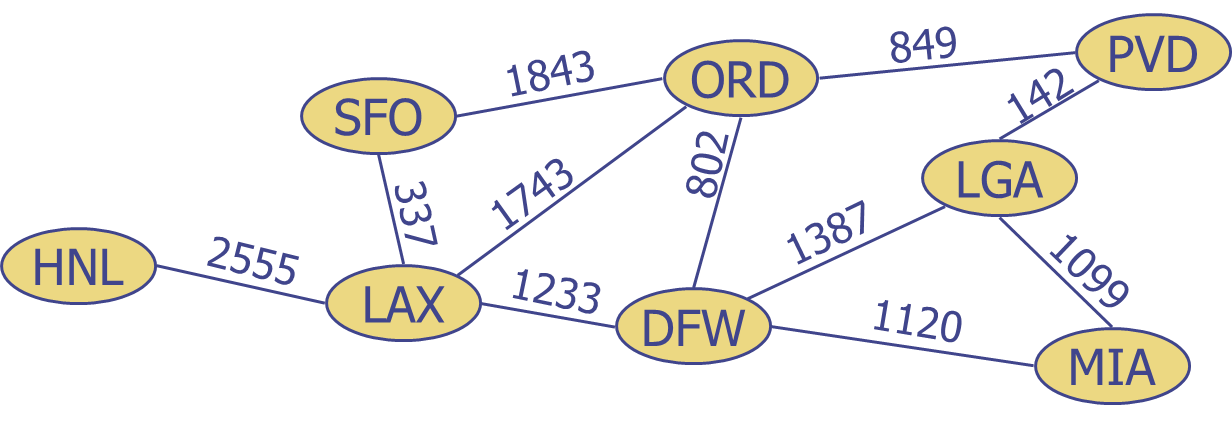
\includegraphics[width=10.5cm]{asp-14-pic01.png}
  \end{center}
\end{frame}

\begin{frame}[fragile]
  \frametitle{Vrste grana}
  \begin{columns}
    \begin{column}[t]{8cm}
      \begin{itemize}
        \item usmerena grana
        \begin{itemize}
          \item uređeni par čvorova $(u,v)$
          \item prvi čvor $u$ je polazište
          \item drugi čvor $v$ je odredište
          \item npr. konkretan let aviona
        \end{itemize}
        \item neusmerena grana
        \begin{itemize}
          \item neuređeni par čvorova $(u,v)$
          \item npr. putanja leta
        \end{itemize}
        \item usmereni graf
        \begin{itemize}
          \item sve grane su usmerene
          \item npr. mreža letova
        \end{itemize}
        \item neusmereni graf
        \begin{itemize}
          \item sve grane su neusmerene
          \item npr. mreža putanja
        \end{itemize}
      \end{itemize}
    \end{column}
    \begin{column}[t]{4cm}
      \begin{center}
        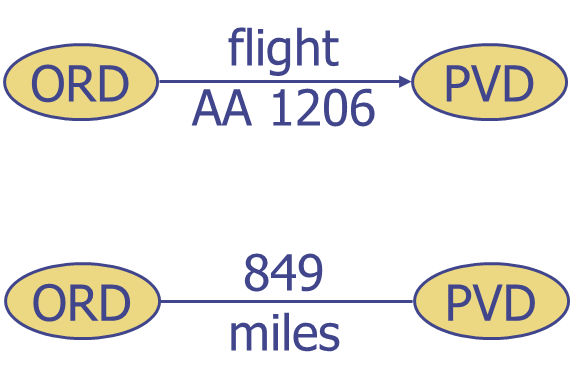
\includegraphics[width=4cm]{asp-14-pic02.png}
      \end{center}
    \end{column}
  \end{columns}
\end{frame}

\begin{frame}[fragile]
  \frametitle{Primene}
  \begin{columns}
    \begin{column}[t]{6cm}
      \begin{itemize}
        \item elektronska kola
        \begin{itemize}
          \item štampane ploče
          \item integrisana kola
        \end{itemize}
        \item transportne mreže
        \begin{itemize}
          \item putevi
          \item avionski letovi
        \end{itemize}
        \item računarske mreže
        \begin{itemize}
          \item lokalne mreže
          \item Internet
        \end{itemize}
        \item baze podataka
        \begin{itemize}
          \item ER dijagrami
        \end{itemize}
      \end{itemize}
    \end{column}
    \begin{column}[t]{6cm}
      \begin{center}
        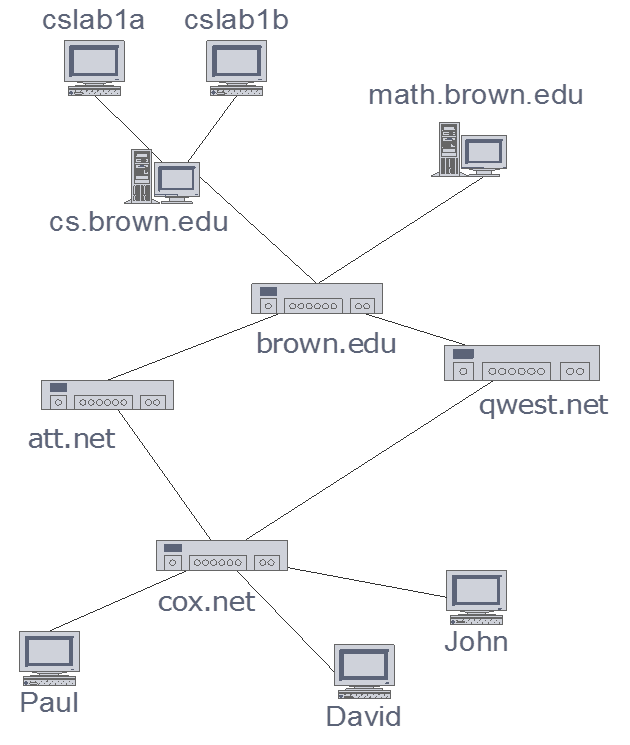
\includegraphics[width=5cm]{asp-14-pic03.png}
      \end{center}
    \end{column}
  \end{columns}
\end{frame}

\begin{frame}[fragile]
  \frametitle{Terminologija $_{1}$}
  \begin{columns}
    \begin{column}[t]{6cm}
      \begin{itemize}
        \item krajevi grane
        \begin{itemize}
          \item $U$ i $V$ su krajevi $a$
        \end{itemize}
        \item grane incidentne na čvoru
        \begin{itemize}
          \item $a$, $d$ i $b$ su incidentni na $V$
        \end{itemize}
        \item susedni čvorovi
        \begin{itemize}
          \item povezani granom
          \item $U$ i $V$ su susedni
        \end{itemize}
        \item stepen čvora
        \begin{itemize}
          \item broj grana kojima je on kraj
          \item stepen of $X$ je 5
        \end{itemize}
        \item paralelne grane: $h$ i $i$
        \item petlja: $j$
      \end{itemize}
    \end{column}
    \begin{column}[t]{6cm}
      \begin{center}
        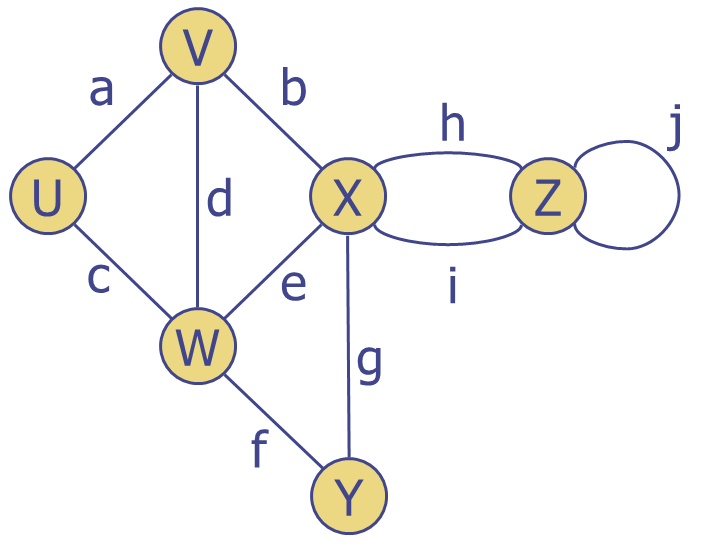
\includegraphics[width=6cm]{asp-14-pic04.png}
      \end{center}
    \end{column}
  \end{columns}
\end{frame}

\begin{frame}[fragile]
  \frametitle{Terminologija $_{2}$}
  \begin{columns}
    \begin{column}[t]{7.5cm}
      \begin{itemize}
        \item putanja
        \begin{itemize}
          \item sekvenca naizmenično čvorova i grana
          \item počinje sa čvorom
          \item završava sa čvorom
          \item svakoj grani prethodi i sledi njen kraj
        \end{itemize}
        \item prosta putanja
        \begin{itemize}
          \item svi čvorovi i grane su različiti
        \end{itemize}
        \item primeri
        \begin{itemize}
          \item $P_{1}=(V,b,X,h,Z)$ je prosta
          \item $P_{2}=(U,c,W,e,X,g,Y,f,W,d,V)$ nije prosta
        \end{itemize}
      \end{itemize}
    \end{column}
    \begin{column}[t]{4.5cm}
      \begin{center}
        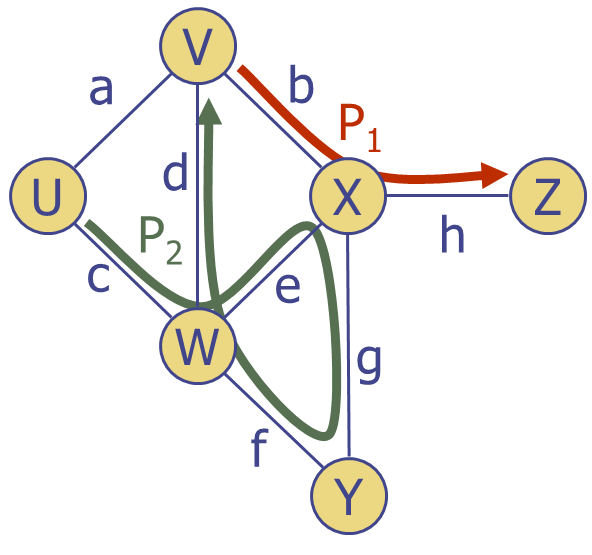
\includegraphics[width=4.5cm]{asp-14-pic05.png}
      \end{center}
    \end{column}
  \end{columns}
\end{frame}

\begin{frame}[fragile]
  \frametitle{Terminologija $_{3}$}
  \begin{columns}
    \begin{column}[t]{9cm}
      \begin{itemize}
        \item petlja
        \begin{itemize}
          \item cirkularna sekvenca naizmenično čvorova i grana
          \item svakoj grani prethodi i sledi njen kraj
        \end{itemize}
        \item prosta petlja
        \begin{itemize}
          \item s vi čvorovi i grane su različiti
        \end{itemize}
        \item primeri
        \begin{itemize}
          \item $C_{1}=(V,b,X,g,Y,f,W,c,U,a,V)$ je prosta
          \item $C_{2}=(U,c,W,e,X,g,Y,f,W,d,V,a,U)$ nije prosta
        \end{itemize}
      \end{itemize}
    \end{column}
    \begin{column}[t]{4.5cm}
      \begin{center}
        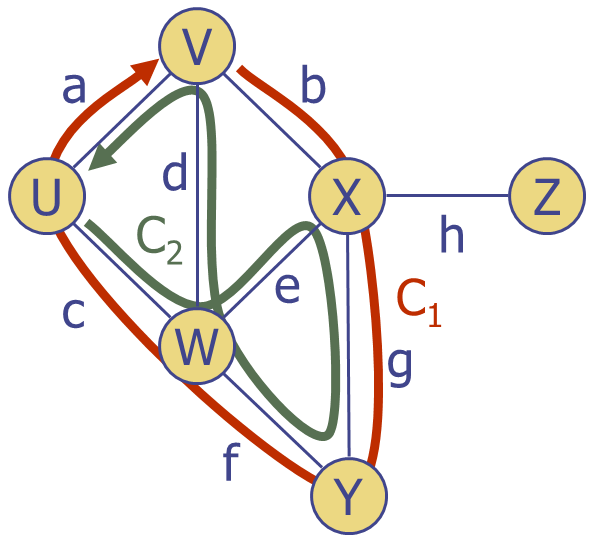
\includegraphics[width=4.5cm]{asp-14-pic06.png}
      \end{center}
    \end{column}
  \end{columns}
\end{frame}

\begin{frame}[fragile]
  \frametitle{Osobine}
  \begin{columns}
    \begin{column}[t]{7.5cm}
      \begin{itemize}
        \item suma stepena čvorova
        $$\sum_{v}deg(v)=2m$$
        (svaka grana se broji dva puta)
        \item u neusmerenom grafu bez petlji i višestrukih grana
        $$m < n(n-1)/2$$
        (svaki čvor ima stepen najviše $n-1$)
      \end{itemize}
    \end{column}
    \begin{column}[t]{4.5cm}
      \begin{itemize}
        \item $n$ -- broj čvorova
        \item $m$ -- broj grana
        \item $deg(v)$ -- stepen čvora
      \end{itemize}
      \begin{center}
        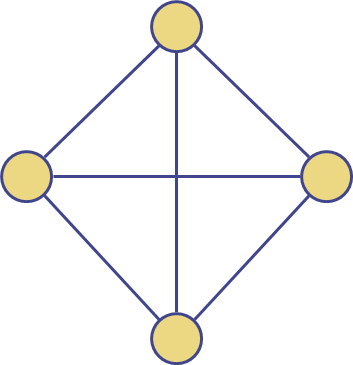
\includegraphics[width=2cm]{asp-14-pic07.png}
      \end{center}
      \begin{itemize}
        \item $n=4$
        \item $m=6$
        \item $deg(v)=3$
      \end{itemize}
    \end{column}
  \end{columns}
\end{frame}

\begin{frame}[fragile]
  \frametitle{Čvorovi i grane}
  \begin{itemize}
    \item graf je kolekcija čvorova i grana
    \item prikazaćemo ga pomoću tri tipa: \texttt{Vertex}, \texttt{Edge} 
    i \texttt{Graph}
    \item \texttt{Vertex} je ,,lagani`` objekat koji čuva sadržaj (npr.
    šifru aerodroma)
    \begin{itemize}
      \item ima metodu \texttt{element()} kojom se može dobiti taj sadržaj
    \end{itemize}
    \item \texttt{Edge} čuva sadržaj (npr. broj leta, rastojanje)
    \begin{itemize}
      \item \texttt{element()} vraća taj sadržaj
      \item \texttt{endpoints()} vraća par $(u,v)$ polazište i odredište
      \item \texttt{opposite(v)} vraća suprotni kraj grane
    \end{itemize}
  \end{itemize}
\end{frame}

\begin{frame}[fragile]
  \frametitle{Graf ATP}
  {%\scriptsize
  \begin{tabular}{r|p{6cm}}
    \texttt{vertex\_count()} & broj čvorova \\ \hline
    \texttt{vertices()} & lista svih čvorova \\ \hline
    \texttt{edge\_count()} & broj grana \\ \hline
    \texttt{edges()} & lista svih grana \\ \hline
    \texttt{get\_edge(u,v)} & vraća granu između \texttt{u} i \texttt{v}
      ako postoji, inače \texttt{None} \\ \hline
    \texttt{degree(v,out=True)} & broj izlaznih/ulaznih grana iz 
      \texttt{v} \\ \hline
    \texttt{incident\_edges(v,out=True)} & lista izlaznih/ulaznih grana 
      iz \texttt{v} \\ \hline
    \texttt{insert\_vertex(x=None)} & dodaj novi čvor sa sadržajem 
      \texttt{x} \\ \hline
    \texttt{insert\_edge(u,v,x=None)} & dodaj novu granu od \texttt{u} 
      ka \texttt{v} sa sadržajem \texttt{x}\\ \hline
    \texttt{remove\_vertex(v)} & ukloni čvor \texttt{v} i sve vezane 
      grane \\ \hline
    \texttt{remove\_edge(e)} & ukloni granu \texttt{e} \\
  \end{tabular}
  }
\end{frame}

\begin{frame}[fragile]
  \frametitle{Implementacija$_1$: Lista čvorova i lista grana}
  \begin{columns}
    \begin{column}[t]{6cm}
      \begin{itemize}
        \item \texttt{Vertex}
        \begin{itemize}
          \item čuva sadržaj
          \item element liste
        \end{itemize}
        \item \texttt{Edge}
        \begin{itemize}
          \item čuva sadržaj
          \item referenca na polazište
          \item referenca na odredište
          \item element liste
        \end{itemize}
        \item lista čvorova
        \item lista grana
      \end{itemize}
    \end{column}
    \begin{column}[t]{6cm}
      \begin{center}
        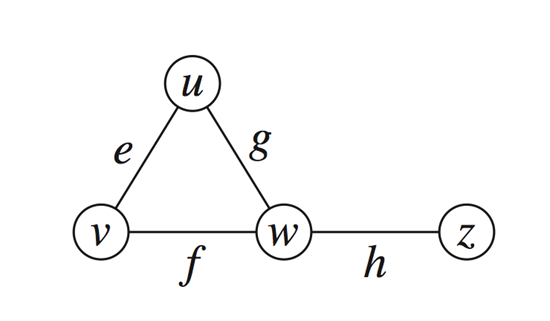
\includegraphics[width=3.5cm]{asp-14-pic08.png} \\
        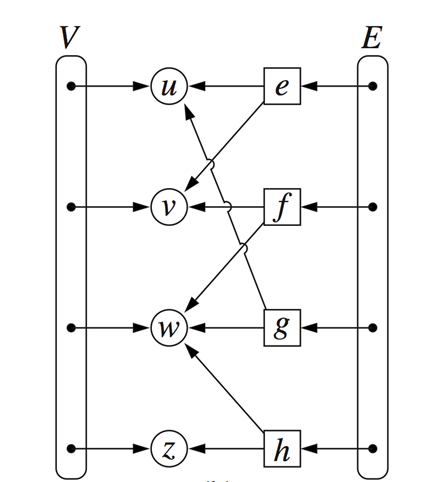
\includegraphics[width=3.5cm]{asp-14-pic09.png}
      \end{center}
    \end{column}
  \end{columns}
\end{frame}

\begin{frame}[fragile]
  \frametitle{Implementacija$_2$: Lista suseda}
  \begin{columns}
    \begin{column}[t]{6cm}
      \begin{itemize}
        \item lista grana za svaki čvor
        \item grane mogu imati reference na drugu pojavu iste grane (za 
          drugi krajnji čvor)
      \end{itemize}
    \end{column}
    \begin{column}[t]{6cm}
      \begin{center}
        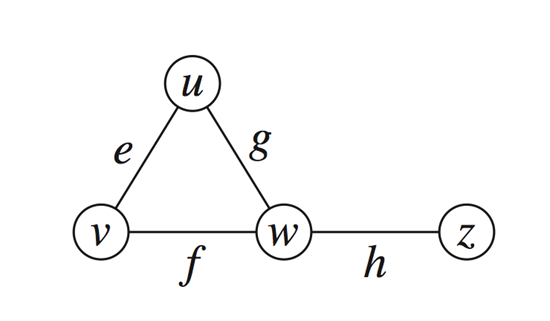
\includegraphics[width=4cm]{asp-14-pic10.png} \\
        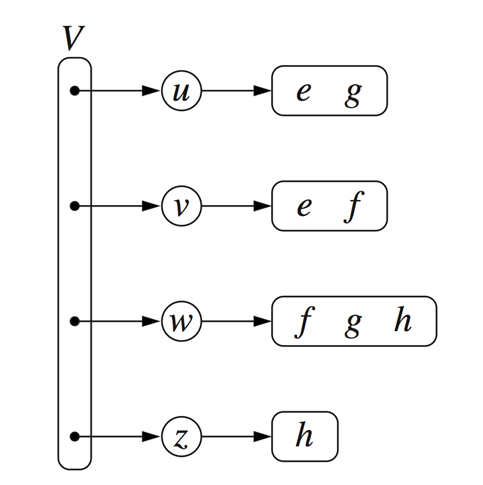
\includegraphics[width=4cm]{asp-14-pic11.png}
      \end{center}
    \end{column}
  \end{columns}
\end{frame}

\begin{frame}[fragile]
  \frametitle{Implementacija$_3$: Matrica incidencije}
  \begin{columns}
    \begin{column}[t]{6cm}
      \begin{itemize}
        \item svakom čvoru dodeljen int ključ
        \item matrica sadrži referencu na granu ukoliko ona povezuje
          dva čvora, ili None
        \item ili samo 0/1 u matrici
      \end{itemize}
    \end{column}
    \begin{column}[t]{6cm}
      \begin{center}
        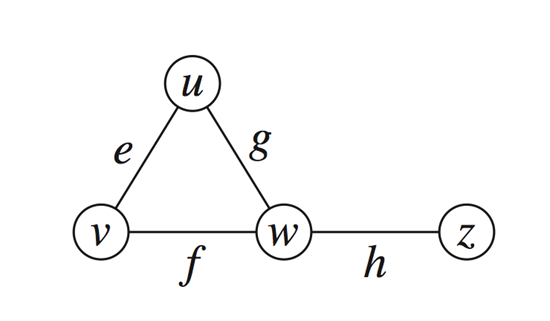
\includegraphics[width=5cm]{asp-14-pic12.png} \\
        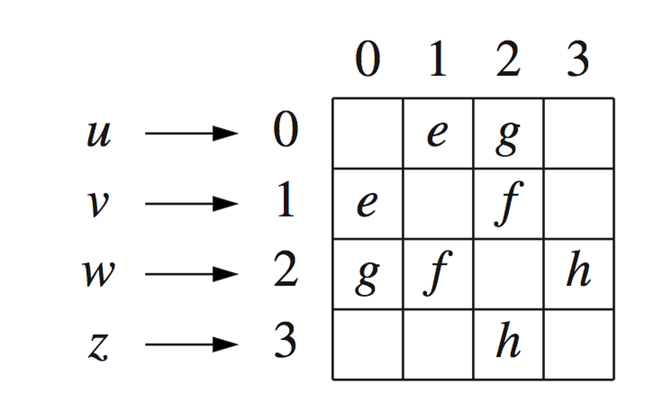
\includegraphics[width=5cm]{asp-14-pic13.png}
      \end{center}
    \end{column}
  \end{columns}
\end{frame}

\begin{frame}[fragile]
  \frametitle{Performanse}
  %\begin{itemize}
    %\item 
    $n$ čvorova, $m$ grana, bez paralelnih grana, bez petlji \\ \ \\
  %\end{itemize}
  %{\scriptsize
  \begin{tabular}{l|c|c|c}
     & lista & lista & matrica \\
     & grana & suseda & incidencije \\ \hline     
    \textit{prostor} & $n+m$ & $n+m$ & $n^2$ \\ \hline
    \texttt{incident\_edges(v)} & $m$ & $deg(v)$ & $n$ \\ \hline
    \texttt{are\_adjacent(v,w)} & $m$ & $\min\{deg(v),deg(w)\}$ & $1$ \\ \hline
    \texttt{insert\_vertex(v)} & $1$ & $1$ & $n^2$ \\ \hline
    \texttt{insert\_edge(v,w,e)} & $1$ & $1$ & $1$ \\ \hline
    \texttt{remove\_vertex(v)} & $m$ & $deg(v)$ & $n^2$ \\ \hline
    \texttt{remove\_edge(e)} & $1$ & $1$ & $1$ \\
  \end{tabular}
  %}
\end{frame}

\begin{frame}[fragile]
  \frametitle{Python implementacija}
  \begin{itemize}
    \item koristićemo mapu susedstva
    \item za čvor $v$ čuvamo Python rečnik sa susedima $I(v)$
    \item listu čvorova zamenićemo rečnikom $D$ koji mapira svaki čvor 
      na njegovu mapu suseda $I(v)$
    \begin{itemize}
      \item možemo proći kroz sve čvorove sa \texttt{D.keys()}
    \end{itemize}
    \item čvor ne mora da čuva svoj položaj u $D$ jer se to izračuna za 
      $O(1)$
    \item performanse iste kao za listu suseda ali u \textbf{očekivanom}
      slučaju
  \end{itemize}
\end{frame}

\begin{frame}[fragile,shrink]
  \frametitle{Klasa Vertex}
\begin{minted}[linenos=false]{python}
class Vertex:
  """Lightweight vertex structure for a graph."""
  __slots__ = '_element'

  def __init__(self, x):
    """Do not call constructor directly. 
    Use Graph's insert_vertex(x).
    """
    self._element = x

  def element(self):
    """Return element associated with this vertex."""
    return self._element

  def __hash__(self):  # will allow vertex to be a map/set key
    return hash(id(self))

  def __str__(self):
    return str(self._element)
\end{minted}
\end{frame}

\begin{frame}[fragile,shrink]
  \frametitle{Klasa Edge}
\begin{minted}[linenos=false]{python}
class Edge:
  __slots__ = '_origin', '_destination', '_element'

  def __init__(self, u, v, x):
    self._origin = u
    self._destination = v
    self._element = x

  def endpoints(self):
    return (self._origin, self._destination)

  def opposite(self, v):
    if not isinstance(v, Graph.Vertex):
      raise TypeError('v must be a Vertex')
    return self._destination if v is self._origin else self._origin
    raise ValueError('v not incident to edge')

  def element(self):
    return self._element

  def __hash__(self):  # will allow edge to be a map/set key
    return hash( (self._origin, self._destination) )

  def __str__(self):
    return '({0},{1},{2})'.format(self._origin,self._destination,self._element)
\end{minted}
\end{frame}

\begin{frame}[fragile,shrink]
  \frametitle{Klasa Graph $_1$}
\begin{minted}[linenos=false]{python}
class Graph:
  def __init__(self, directed=False):
    self._outgoing = {}
    self._incoming = {} if directed else self._outgoing

  def _validate_vertex(self, v):
    if not isinstance(v, self.Vertex):
      raise TypeError('Vertex expected')
    if v not in self._outgoing:
      raise ValueError('Vertex does not belong to this graph.')
    
  def is_directed(self):
    return self._incoming is not self._outgoing

  def vertex_count(self):
    return len(self._outgoing)

  def vertices(self):
    return self._outgoing.keys()
\end{minted}
\end{frame}

\begin{frame}[fragile,shrink]
  \frametitle{Klasa Graph $_2$}
\begin{minted}[linenos=false]{python}
  def edge_count(self):
    total = sum(len(self._outgoing[v]) for v in self._outgoing)
    return total if self.is_directed() else total // 2

  def edges(self):
    result = set() # avoid double-reporting edges of undirected graph
    for secondary_map in self._outgoing.values():
      result.update(secondary_map.values()) # add edges to resulting set
    return result

  def get_edge(self, u, v):
    self._validate_vertex(u)
    self._validate_vertex(v)
    return self._outgoing[u].get(v) # returns None if v not adjacent

  def degree(self, v, outgoing=True):   
    self._validate_vertex(v)
    adj = self._outgoing if outgoing else self._incoming
    return len(adj[v])
\end{minted}
\end{frame}

\begin{frame}[fragile,shrink]
  \frametitle{Klasa Graph $_3$}
\begin{minted}[linenos=false]{python}
  def incident_edges(self, v, outgoing=True):   
    self._validate_vertex(v)
    adj = self._outgoing if outgoing else self._incoming
    for edge in adj[v].values():
      yield edge

  def insert_vertex(self, x=None):
    v = self.Vertex(x)
    self._outgoing[v] = {}
    if self.is_directed():
      self._incoming[v] = {} # need distinct map for incoming edges
    return v
      
  def insert_edge(self, u, v, x=None):
    if self.get_edge(u, v) is not None:  # includes error checking
      raise ValueError('u and v are already adjacent')
    e = self.Edge(u, v, x)
    self._outgoing[u][v] = e
    self._incoming[v][u] = e
\end{minted}
\end{frame}

\begin{frame}[fragile]
  \frametitle{Podgraf}
  \begin{columns}
    \begin{column}[t]{6cm}
      \begin{itemize}
        \item \myred{podgraf} $S$ grafa $G$ je graf takav da
        \begin{itemize}
          \item čvorovi $S$ su podskup čvorova $G$
          \item grane $S$ su podskup grana $G$ \\ \ \\
        \end{itemize}
        \item \myred{pokrivajući podgraf} sadrži sve čvorove $G$
      \end{itemize}
    \end{column}
    \begin{column}[t]{6cm}
      \begin{center}
        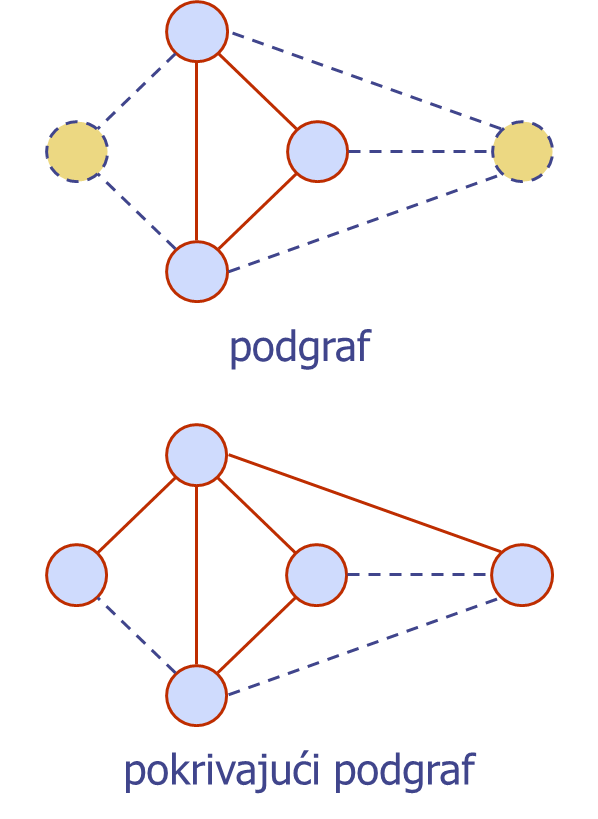
\includegraphics[width=4cm]{asp-14-pic14.png}
      \end{center}
    \end{column}
  \end{columns}
\end{frame}

\begin{frame}[fragile]
  \frametitle{Povezanost}
  \begin{columns}
    \begin{column}[t]{6cm}
      \begin{itemize}
        \item graf je \myred{povezan} ako postoji putanja između svaka 
          dva čvora
        \item \myred{povezana komponenta} je maksimalni povezani podgraf
      \end{itemize}
    \end{column}
    \begin{column}[t]{6cm}
      \begin{center}
        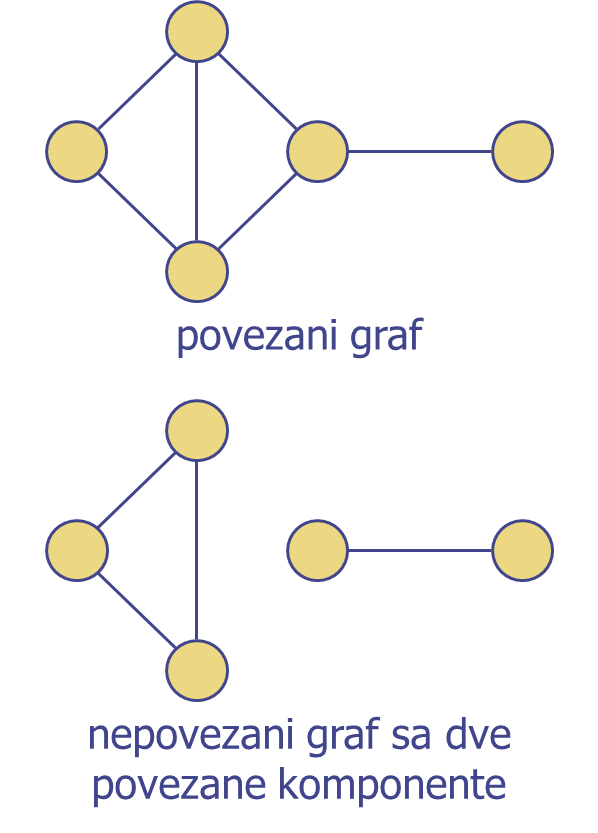
\includegraphics[width=4.5cm]{asp-14-pic15.png}
      \end{center}
    \end{column}
  \end{columns}
\end{frame}

\begin{frame}[fragile]
  \frametitle{Stablo i šuma}
  \begin{columns}
    \begin{column}[t]{6cm}
      \begin{itemize}
        \item \myred{stablo} je neusmereni graf $T$ takav da
        \begin{itemize}
          \item $T$ je povezan
          \item $T$ nema petlje
        \end{itemize}
        \item \myred{šuma} je neusmereni graf takav da
        \begin{itemize}
          \item nema petlje
          \item povezane komponente su stabla
        \end{itemize}
      \end{itemize}
    \end{column}
    \begin{column}[t]{6cm}
      \begin{center}
        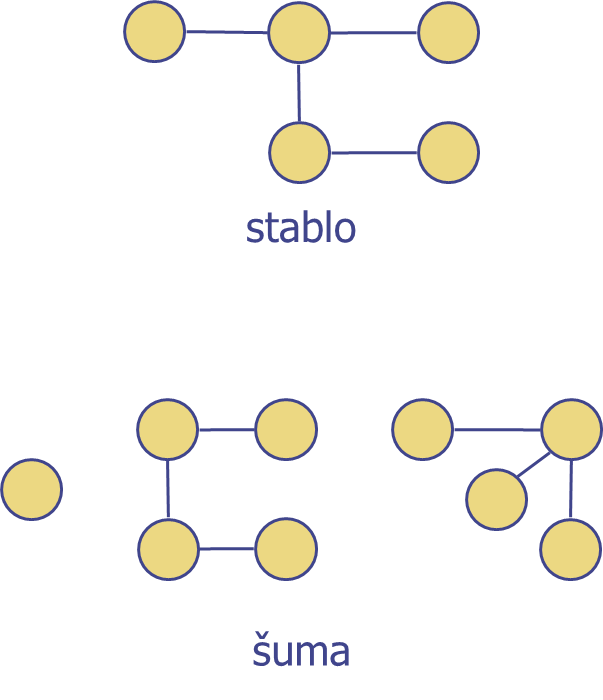
\includegraphics[width=5cm]{asp-14-pic16.png}
      \end{center}
    \end{column}
  \end{columns}
\end{frame}

\begin{frame}[fragile]
  \frametitle{Pokrivajuće stablo i šuma}
  \begin{columns}
    \begin{column}[t]{6cm}
      \begin{itemize}
        \item \myred{pokrivajuće stablo} je podgraf koji
        \begin{itemize}
          \item je stablo i
          \item pokriva graf
        \end{itemize}
        \item pokrivajuće stablo nije jedinstveno ako graf nije stablo
        \item \myred{pokrivajuća šuma} je podgraf koji
        \begin{itemize}
          \item je šuma i
          \item pokriva graf
        \end{itemize}
      \end{itemize}
    \end{column}
    \begin{column}[t]{6cm}
      \begin{center}
        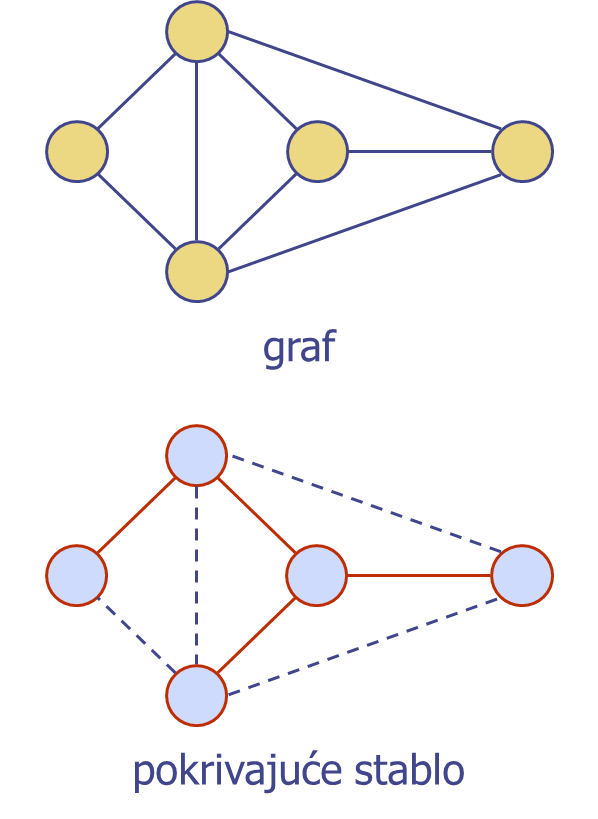
\includegraphics[width=4.5cm]{asp-14-pic17.png}
      \end{center}
    \end{column}
  \end{columns}
\end{frame}

\section[Obilazak grafa]{Obilazak grafa}

\begin{frame}[fragile]
  \frametitle{Obilazak grafa po dubini}
  \begin{columns}
    \begin{column}[t]{8cm}
      \begin{itemize}
        \item depth-first-search (\myred{DFS}) je opšti metod za 
        obilazak grafa
        \begin{itemize}
          \item obilazi sve čvorove i grane
          \item određuje da li je graf povezan
          \item određuje povezane komponente grafa
          \item određuje pokrivajuću šumu grafa
        \end{itemize}
      \end{itemize}
    \end{column}
    \begin{column}[t]{8cm}
      \begin{itemize}
        \item DFS na grafu sa $n$ čvorova i $m$ grana traje $O(n+m)$
        \item može se proširiti za rešavanje drugih problema
        \begin{itemize}
          \item nađi putanju između dva čvora
          \item nađi petlju u grafu
        \end{itemize}
        \item DFS je za graf isto što i Ojlerov obilazak za binarna 
          stabla
      \end{itemize}
    \end{column}
  \end{columns}
\end{frame}

\begin{frame}[fragile]
  \frametitle{DFS algoritam}
  dodeljuje oznake (labele) čvorovima i granama
  {\footnotesize
  \begin{columns}
    \begin{column}[t]{8cm}
      \begin{algorithmic}
        \STATE \myred{DFS}($G$)
        \REQUIRE graf $G$
        \ENSURE oznake na granama: {\scriptsize DISCOVERY} ili {\scriptsize BACK}
        \FORALL{$u\in G$.vertices()}
          \STATE setLabel($u$, {\scriptsize UNEXPLORED})
        \ENDFOR
        \FORALL{$e\in G$.edges()}
          \STATE setLabel($e$, {\scriptsize UNEXPLORED})
        \ENDFOR
        \FORALL{$v\in G$.vertices()}
          \IF{label($v$) = {\scriptsize UNEXPLORED}}
            \STATE DFS($G,v$)
          \ENDIF
        \ENDFOR
      \end{algorithmic}
    \end{column}
    \begin{column}[t]{8cm}
      \begin{algorithmic}
        \STATE \myred{DFS}($G,v$)
        \REQUIRE graf $G$ i početni čvor $v$
        \ENSURE oznake na granama: {\scriptsize DISCOVERY} ili {\scriptsize BACK}
        \STATE setLabel($v$, {\scriptsize VISITED})
        \FORALL{$e\in G$.incidentEdges($v$)}
          \IF{label($e$) = {\scriptsize UNEXPLORED}}
            \STATE $w \leftarrow$ opposite($v,e$)
            \IF{label($w$) = {\scriptsize UNEXPLORED}}
              \STATE setLabel($e$, {\scriptsize DISCOVERY})
              \STATE DFS($G, w$)
            \ELSE
              \STATE setLabel($e$, {\scriptsize BACK})
            \ENDIF
          \ENDIF
        \ENDFOR
      \end{algorithmic}
    \end{column}
  \end{columns}
  }
\end{frame}

\begin{frame}[fragile,shrink=15]
  \frametitle{DFS u Pythonu}
\begin{minted}[linenos=false]{python}
def DFS(g, u, discovered):
  for e in g.incident_edges(u): # for every outgoing edge from u
    v = e.opposite(u)
    if v not in discovered:  # v is an unvisited vertex
      discovered[v] = e      # e is the tree edge that discovered v
      DFS(g, v, discovered)  # recursively explore from v
\end{minted}
\end{frame}

\begin{frame}[fragile]
  \frametitle{DFS primer}
  \begin{center}
    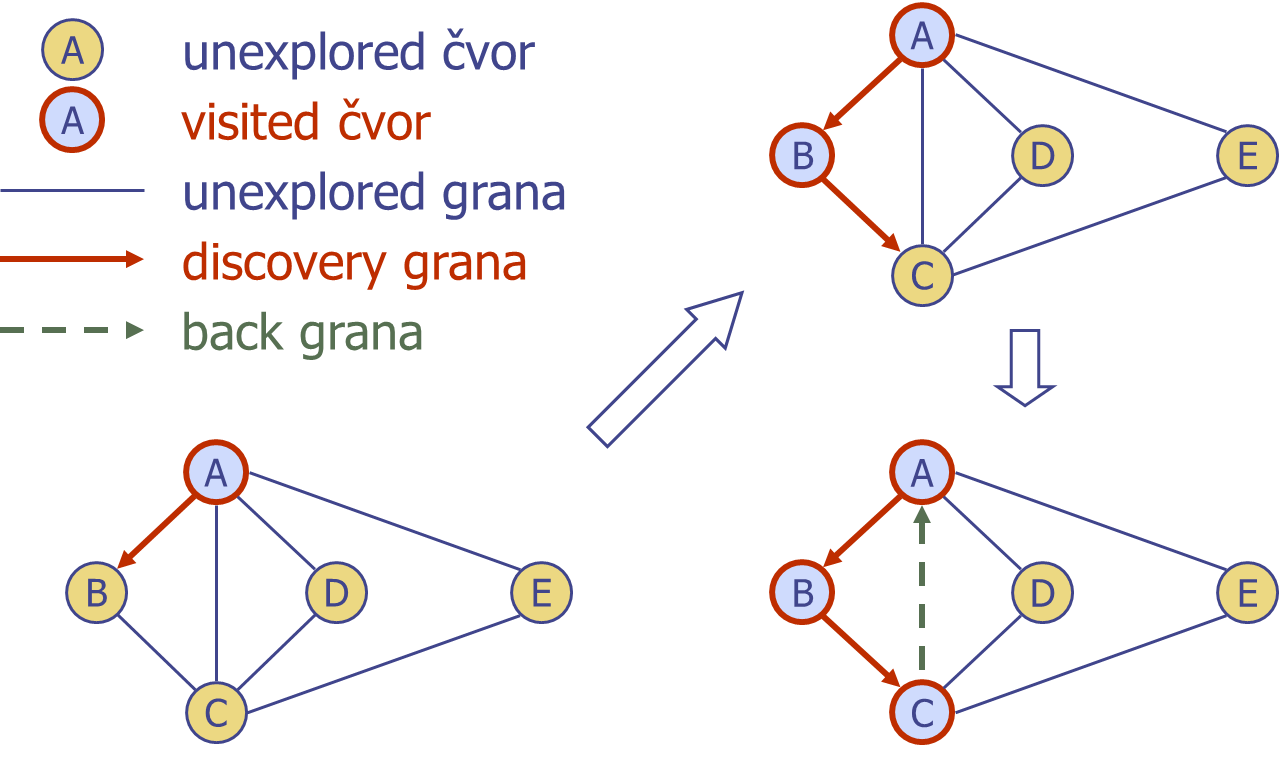
\includegraphics[width=11cm]{asp-14-pic18.png}
  \end{center}
\end{frame}

\begin{frame}[fragile]
  \frametitle{DFS primer (još)}
  \begin{center}
    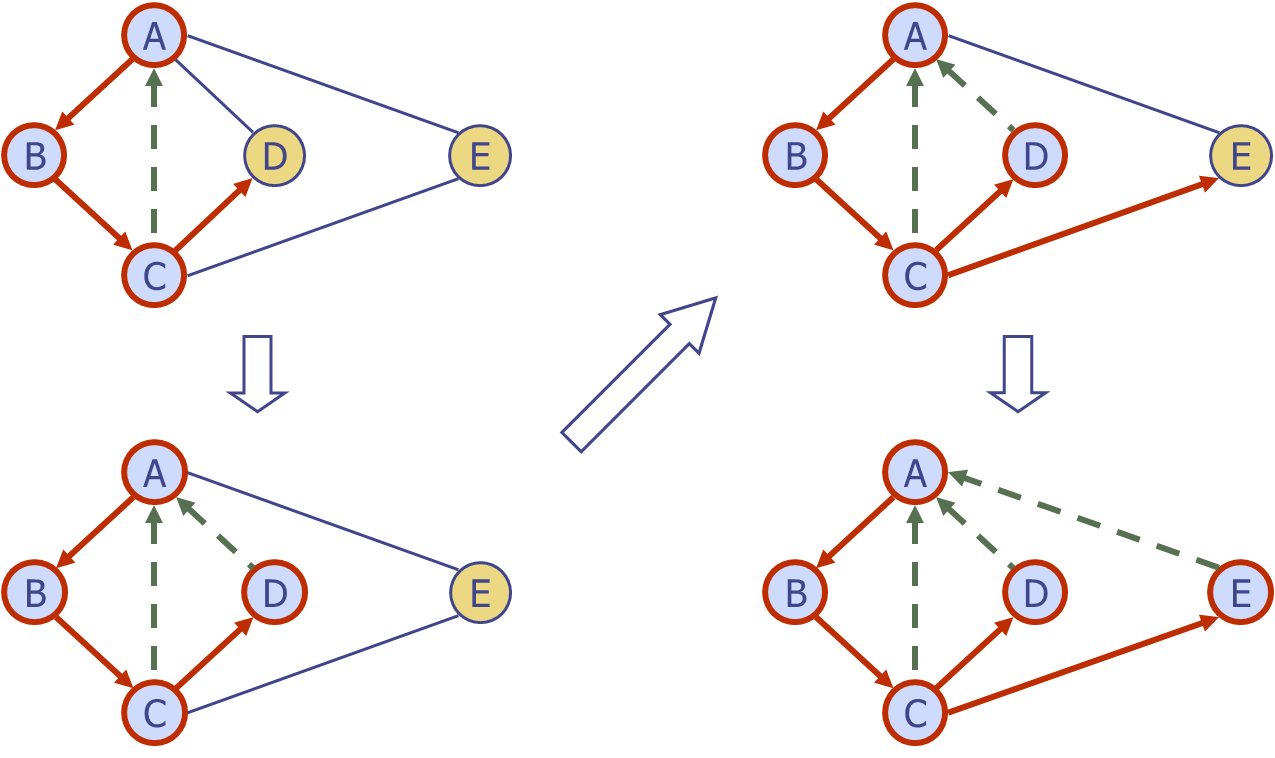
\includegraphics[width=11cm]{asp-14-pic19.png}
  \end{center}
\end{frame}

\begin{frame}[fragile]
  \frametitle{DFS i prolazak lavirinta}
  \begin{columns}
    \begin{column}[t]{6cm}
      \begin{itemize}
        \item svaku raskrsnicu, ugao (skretanje) i kraj puta označimo
          kao posećen čvor
        \item svaki hodnik (granu) kao posećenu
        \item pamtimo odakle smo počeli pomoću steka rekurzije
      \end{itemize}
    \end{column}
    \begin{column}[t]{6cm}
      \begin{center}
        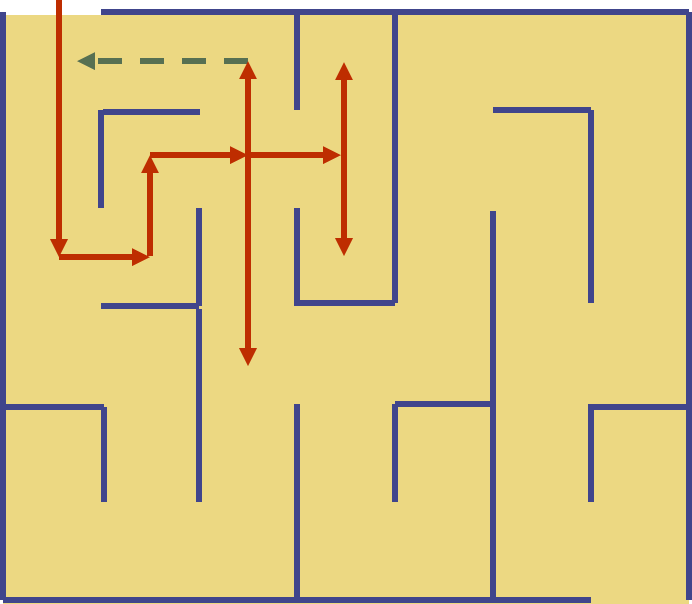
\includegraphics[width=6cm]{asp-14-pic20.png}
      \end{center}
    \end{column}
  \end{columns}
\end{frame}

\begin{frame}[fragile]
  \frametitle{Osobine DFS}
  \begin{columns}
    \begin{column}[t]{6cm}
      \begin{itemize}
        \item[1] DFS($G,v$) obilazi sve čvorove i grane u povezanoj 
          komponenti od $v$
        \item[2] grane označene kao {\scriptsize DISCOVERY} čine 
          pokrivajuće stablo povezane komponente od $v$
      \end{itemize}
    \end{column}
    \begin{column}[t]{6cm}
      \begin{center}
        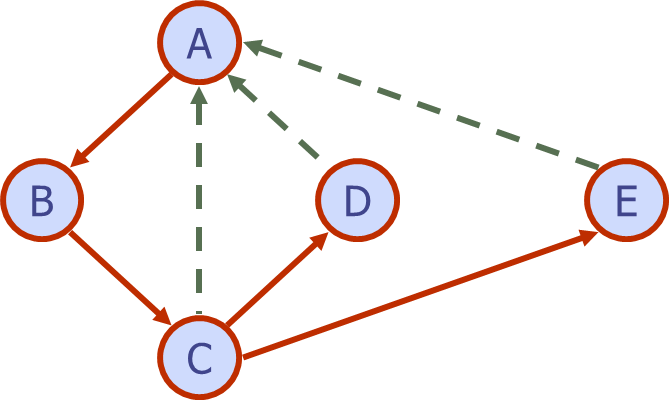
\includegraphics[width=5cm]{asp-14-pic21.png}
      \end{center}
    \end{column}
  \end{columns}
\end{frame}

\begin{frame}[fragile]
  \frametitle{Performanse DFS}
  \begin{itemize}
    \item stavljanje labele na čvor/granu traje $O(1)$
    \item svaki čvor se označi \textbf{dva} puta, jednom kao {\scriptsize 
      UNEXPLORED}, drugi put kao {\scriptsize VISITED}
    \item svaka grana se označi \textbf{dva} puta, jednom kao {\scriptsize 
      UNEXPLORED}, drugi put kao {\scriptsize DISCOVERY} ili 
      {\scriptsize BACK}
    \item metoda \texttt{incident\_edges} se poziva jednom za svaki čvor
    \item DFS traje $O(n+m)$ ako je graf predstavljen listom suseda
    $$\sum_{v}deg(v)=2m$$
  \end{itemize}
\end{frame}

\begin{frame}[fragile]
  \frametitle{DFS za pronalaženje putanje}
  {\footnotesize
  \begin{columns}
    \begin{column}[t]{8cm}
      \begin{itemize}
        \item DFS se može upotrebiti za pronalaženje \textbf{putanje} 
          između dva čvora $u$ i $z$
        \item pozivamo DFS sa $u$ kao početnim čvorom
        \item discovery grane definišu pokrivajuće stablo: postoji putanja od $u$ do $z$
        \item na steku $S$ čuvamo grane od početnog do tekućeg čvora
        \item kada dođemo do $z$ na steku je cela putanja
      \end{itemize}
    \end{column}
    \begin{column}[t]{8cm}
      \begin{algorithmic}
        \STATE \myred{pathDFS}($G,v,z$)
        \STATE setLabel($v$, {\scriptsize VISITED})
        \IF{$v=z$}
          \RETURN $S$.elements()
        \ENDIF
        \FORALL{$e\in G$.incidentEdges($v$)}
          \IF{label($e$) = {\scriptsize UNEXPLORED}}
            \STATE $w \leftarrow$ opposite($v,e$)
            \IF{label($w$) = {\scriptsize UNEXPLORED}}
              \STATE setLabel($e$, {\scriptsize DISCOVERY})
              \STATE $S$.push($e$)
              \STATE pathDFS($G, w$)
              \STATE $S$.pop($e$)
            \ELSE
              \STATE setLabel($e$, {\scriptsize BACK})
            \ENDIF
          \ENDIF
        \ENDFOR
      \end{algorithmic}
    \end{column}
  \end{columns}
  }
\end{frame}

\begin{frame}[fragile,shrink=3]
  \frametitle{DFS za pronalaženje petlje}
  {\footnotesize
  \begin{columns}
    \begin{column}[t]{8cm}
      \begin{itemize}
        \item DFS se može upotrebiti za pronalaženje \textbf{petlje} 
        \item na steku $S$ čuvamo putanju od početnog do tekućeg čvora
        \item čim naiđemo na {\scriptsize BACK} granu $(v,w)$ vraćamo
          petlju kao sadržaj steka od vrha do čvora $w$
      \end{itemize}
    \end{column}
    \begin{column}[t]{8cm}
      \begin{algorithmic}
        \STATE \myred{cycleDFS}($G,v$)
        \STATE setLabel($v$, {\scriptsize VISITED})
        \FORALL{$e\in G$.incidentEdges($v$)}
          \IF{label($e$) = {\scriptsize UNEXPLORED}}
            \STATE $w \leftarrow$ opposite($v,e$)
            \STATE $S$.push($e$)
            \IF{label($w$) = {\scriptsize UNEXPLORED}}
              \STATE setLabel($e$, {\scriptsize DISCOVERY})
              \STATE pathDFS($G, w$)
              \STATE $S$.pop($e$)
            \ELSE
              \STATE $T \leftarrow$ new Stack
              \REPEAT
                \STATE $o \leftarrow S$.pop()
                \STATE $T$.push($o$)
              \UNTIL{$o=w$}
              \RETURN $T$.elements()
            \ENDIF
          \ENDIF
        \ENDFOR
      \end{algorithmic}
    \end{column}
  \end{columns}
  }
\end{frame}


\begin{frame}[fragile]
  \frametitle{Obilazak grafa po širini}
  \begin{columns}
    \begin{column}[t]{8cm}
      \begin{itemize}
        \item breadth-first-search (\myred{BFS}) je opšti metod za 
        obilazak grafa
        \begin{itemize}
          \item obilazi sve čvorove i grane
          \item određuje da li je graf povezan
          \item određuje povezane komponente grafa
          \item određuje pokrivajuću šumu grafa
        \end{itemize}
      \end{itemize}
    \end{column}
    \begin{column}[t]{8cm}
      \begin{itemize}
        \item BFS na grafu sa $n$ čvorova i $m$ grana traje $O(n+m)$
        \item može se proširiti za rešavanje drugih problema
        \begin{itemize}
          \item nađi najkraću putanju između dva čvora
          \item nađi prostu petlju
        \end{itemize}
      \end{itemize}
    \end{column}
  \end{columns}
\end{frame}

\begin{frame}[fragile,shrink=2]
  \frametitle{BFS algoritam}
  {\footnotesize
  \begin{columns}
    \begin{column}[t]{5cm}
      \begin{algorithmic}
        \STATE \myred{BFS}($G$)
        \FORALL{$u\in G$.vertices()}
          \STATE setLabel($u$, {\scriptsize UNEXPLORED})
        \ENDFOR
        \FORALL{$e\in G$.edges()}
          \STATE setLabel($e$, {\scriptsize UNEXPLORED})
        \ENDFOR
        \FORALL{$v\in G$.vertices()}
          \IF{label($v$) = {\scriptsize UNEXPLORED}}
            \STATE BFS($G,v$)
          \ENDIF
        \ENDFOR
      \end{algorithmic}
    \end{column}
    \begin{column}[t]{7cm}
      \begin{algorithmic}
        \STATE \myred{BFS}($G,s$)
        \STATE $L_{0} \leftarrow [\,]$
        \STATE $L_{0}$.addLast($s$)
        \STATE setLabel($s$, {\scriptsize VISITED})
        \STATE $i \leftarrow 0$
        \WHILE{$\neg L_{i}$.isEmpty()}
          \STATE $L_{i+1} \leftarrow [\,]$
          \FORALL{$v \in L_i$.elements()}
            \FORALL{$e \in G$.incidentEdges($v$)}
              \IF{label($e$) = {\scriptsize UNEXPLORED}}
                \STATE $w \leftarrow$ opposite($v,e$)
                \IF{label($w$) = {\scriptsize UNEXPLORED}}
                  \STATE setLabel($e$, {\scriptsize DISCOVERY})
                  \STATE setLabel($w$, {\scriptsize VISITED})
                  \STATE $L_{i+1}$.addLast($w$)
                \ELSE
                  \STATE setLabel($e$, {\scriptsize CROSS})
                \ENDIF
              \ENDIF
            \ENDFOR
          \ENDFOR
          $i \leftarrow i + 1$
        \ENDWHILE
      \end{algorithmic}
    \end{column}
  \end{columns}
  }

  \ %

\end{frame}

\begin{frame}[fragile,shrink=20]
  \frametitle{BFS u Pythonu}
\begin{minted}[linenos=false]{python}
def BFS(g, s, discovered):
  level = [s]        # first level includes only s
  while len(level) > 0:
    next_level = []  # prepare to gather newly found vertices
    for u in level:
      for e in g.incident_edges(u): # for every outgoing edge from u
        v = e.opposite(u)
        if v not in discovered: # v is an unvisited vertex
          discovered[v] = e     # e is the tree edge that discovered v
          next_level.append(v)  # v will be considered in next pass
    level = next_level          # relabel 'next' level to become current
\end{minted}
\end{frame}

\begin{frame}[fragile]
  \frametitle{BFS primer}
  \begin{center}
    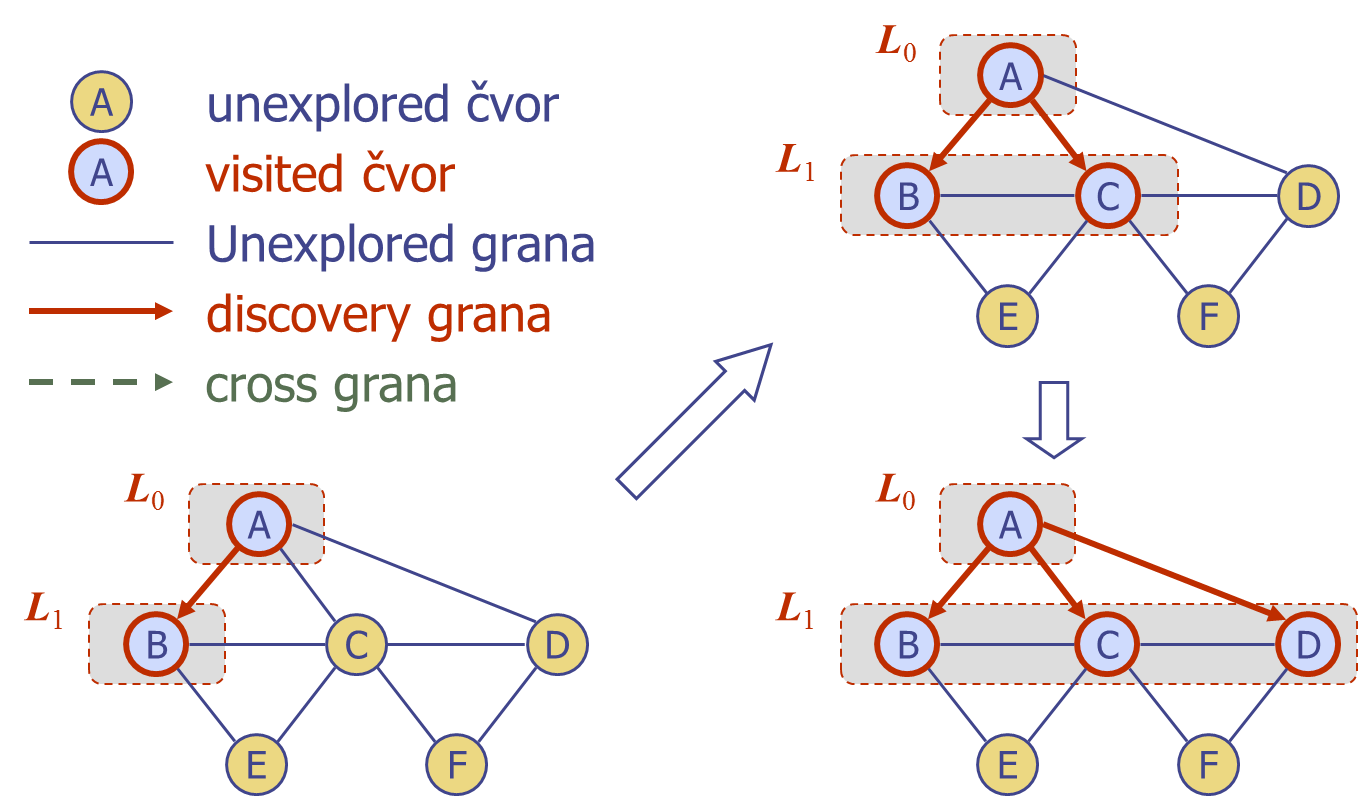
\includegraphics[width=11cm]{asp-14-pic22.png}
  \end{center}
\end{frame}

\begin{frame}[fragile]
  \frametitle{BFS primer (još)}
  \begin{center}
    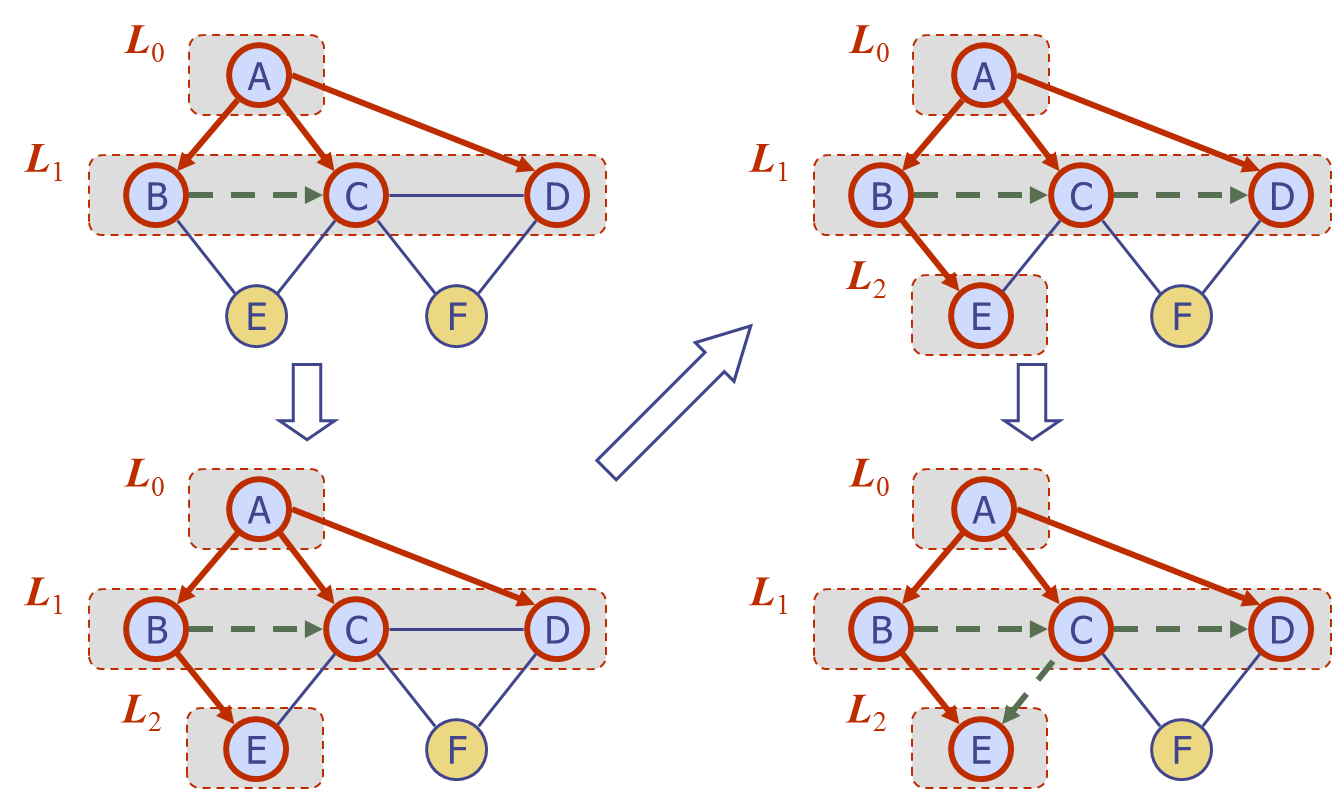
\includegraphics[width=11cm]{asp-14-pic23.png}
  \end{center}
\end{frame}

\begin{frame}[fragile]
  \frametitle{BFS primer (još još)}
  \begin{center}
    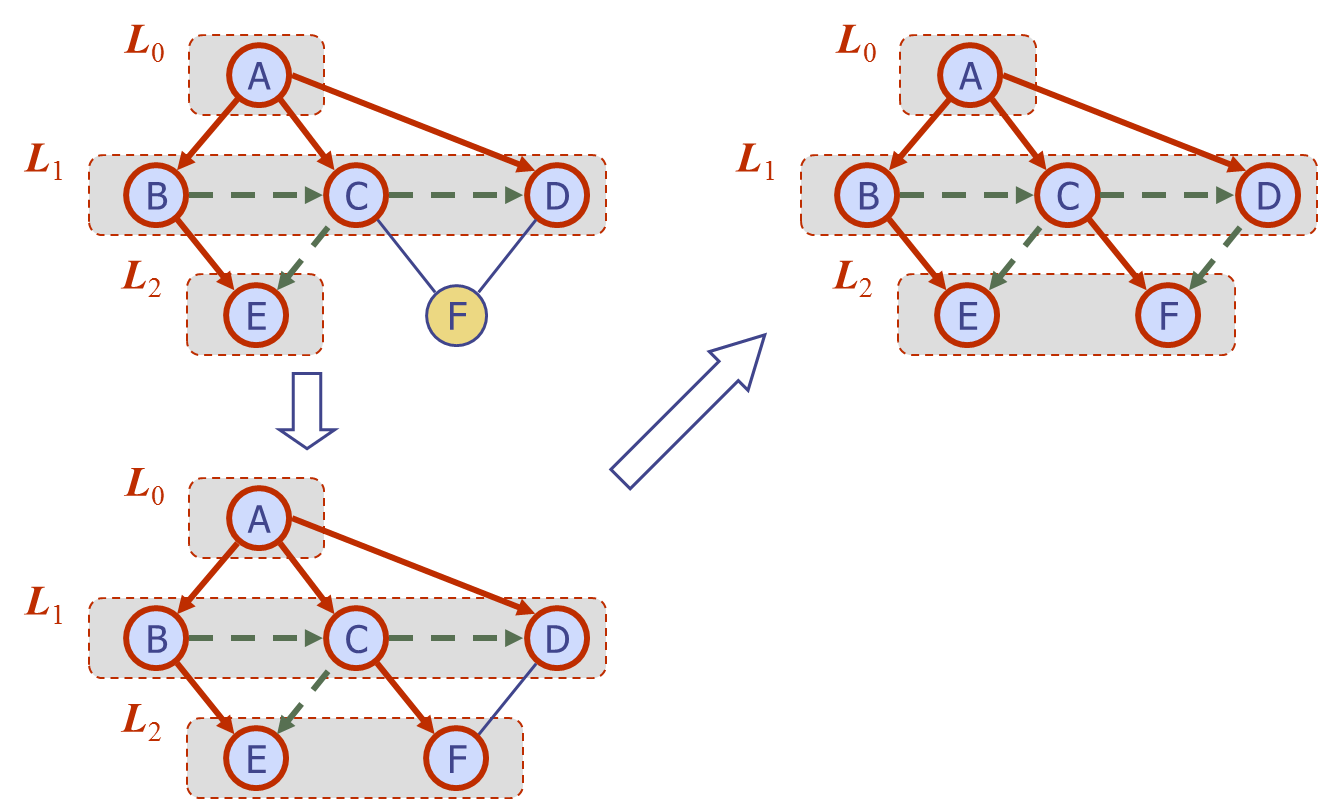
\includegraphics[width=11cm]{asp-14-pic24.png}
  \end{center}
\end{frame}

\begin{frame}[fragile]
  \frametitle{Osobine BFS}
  $G_{s}$: povezana komponenta od $s$
  \begin{columns}
    \begin{column}[t]{9cm}
      \begin{itemize}
        \item[1] BFS($G,v$) obilazi sve čvorove i grane od $G_{s}$
        \item[2] grane označene kao {\scriptsize DISCOVERY} čine 
          pokrivajuće stablo $T_{s}$ za $G_{s}$
        \item[3] za svaki čvor u $L_{i}$
        \begin{itemize}
          \item putanja iz $T_{s}$ od $s$ do $v$ ima $i$ čvorova
          \item svaka putanja od $s$ do $v$ u $G_{s}$ ima bar $i$ čvorova
        \end{itemize}
      \end{itemize}
    \end{column}
    \begin{column}[t]{6cm}
      \begin{center}
        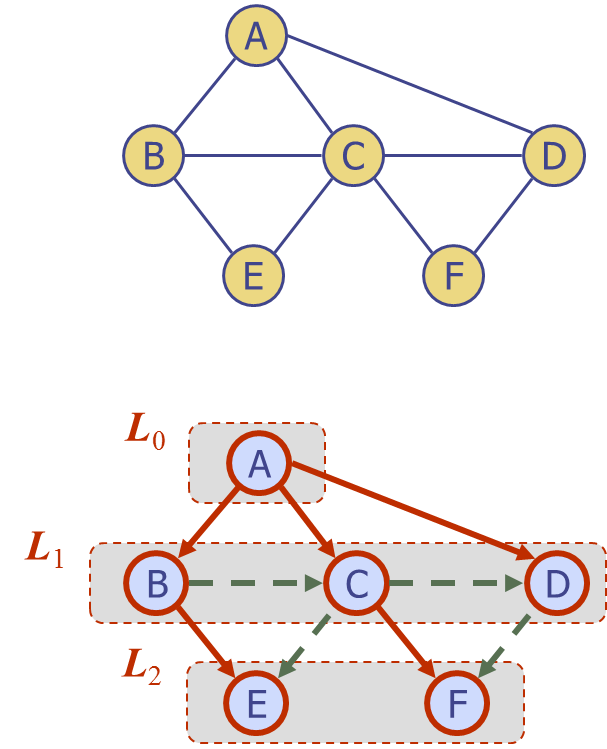
\includegraphics[width=4.5cm]{asp-14-pic25.png}
      \end{center}
    \end{column}
  \end{columns}
\end{frame}

\begin{frame}[fragile]
  \frametitle{Performanse BFS}
  \begin{itemize}
    \item stavljanje labele na čvor/granu traje $O(1)$
    \item svaki čvor se označi \textbf{dva} puta, jednom kao {\scriptsize 
      UNEXPLORED}, drugi put kao {\scriptsize VISITED}
    \item svaka grana se označi \textbf{dva} puta, jednom kao {\scriptsize 
      UNEXPLORED}, drugi put kao {\scriptsize DISCOVERY} ili 
      {\scriptsize CROSS}
    \item svaki čvor se jednom dodaje u sekvencu $L_{i}$
    \item metoda \texttt{incident\_edges} se poziva jednom za svaki čvor
    \item BFS traje $O(n+m)$ ako je graf predstavljen listom suseda
    $$\sum_{v}deg(v)=2m$$
  \end{itemize}
\end{frame}

\begin{frame}[fragile]
  \frametitle{Primene BFS}
  \begin{itemize}
    \item možemo prilagoditi BFS za rešavanje sledećih problema u 
      trajanju $O(n+m)$:
    \begin{itemize}
      \item određivanje povezanih komponenti
      \item određivanje pokrivajuće šume
      \item pronalaženje proste petlje ili je graf šuma
      \item pronalaženje najkraće putanje između dva čvora, ili ne 
        postoji
    \end{itemize}
  \end{itemize}
\end{frame}

\begin{frame}[fragile]
  \frametitle{DFS vs BFS}
  \begin{center}
    \begin{tabular}{l|c|c}
      \textbf{primena} & \textbf{DFS} & \textbf{BFS} \\ \hline
      pokrivajuća šuma, &  &  \\
      povezane komponente, & $\checkmark$ & $\checkmark$ \\
      putanje, petlje &  &  \\ \hline
      najkraći put &  & $\checkmark$ \\ \hline
      bipovezane komponente & $\checkmark$ & \\
    \end{tabular}
    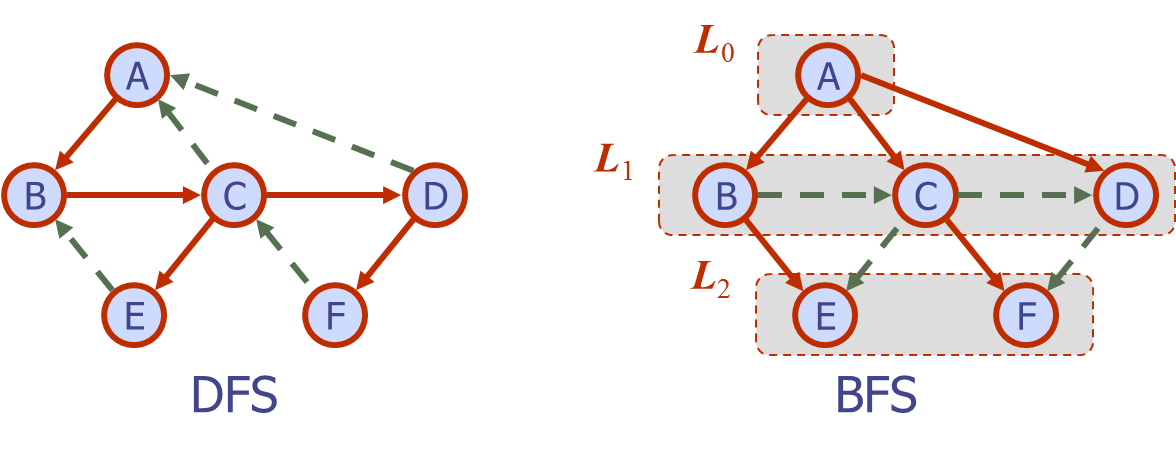
\includegraphics[width=10cm]{asp-14-pic26.png}
  \end{center}
\end{frame}

\begin{frame}[fragile]
  \frametitle{DFS vs BFS}
  \begin{columns}
    \begin{column}[t]{6cm}
      {\scriptsize BACK} grana $(v,w)$
      \begin{itemize}
        \item $w$ je predak od $v$ u stablu koje čine {\scriptsize 
          DISCOVERY} grane
      \end{itemize}
    \end{column}
    \begin{column}[t]{6cm}
      {\scriptsize CROSS} grana $(v,w)$
      \begin{itemize}
        \item $w$ je na istom nivou ili na sledećem nivou u odnosu na 
          $v$
      \end{itemize}
    \end{column}
  \end{columns}
  \begin{center}
    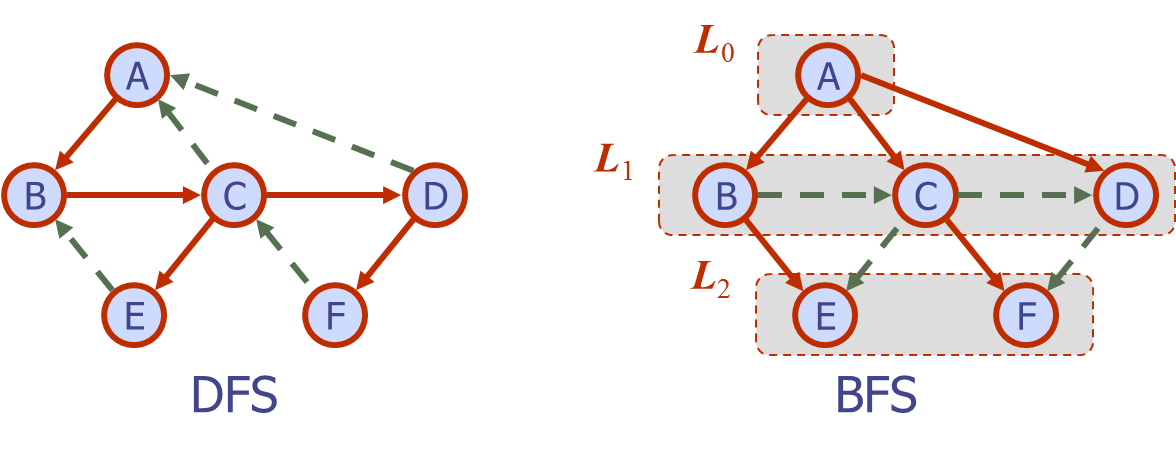
\includegraphics[width=10cm]{asp-14-pic26.png}
  \end{center}
\end{frame}

\section[Usmereni graf]{Usmereni graf i najkraći put}

\begin{frame}[fragile]
  \frametitle{Usmereni graf}
  \begin{columns}
    \begin{column}[t]{6cm}
      \begin{itemize}
        \item \myred{usmereni graf} (directed graph, ,,digraph``) je 
          graf čije su sve grane usmerene
      \end{itemize}
    \end{column}
    \begin{column}[t]{6cm}
      \begin{center}
        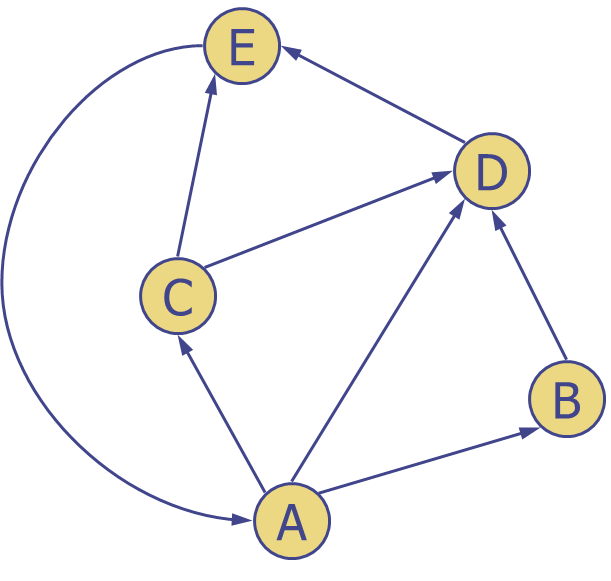
\includegraphics[width=5cm]{asp-14-pic28.png}
      \end{center}
    \end{column}
  \end{columns}
\end{frame}

\begin{frame}[fragile]
  \frametitle{Osobine usmerenog grafa}
  \begin{itemize}
    \item graf $G=(V,E)$ takav da
    \begin{itemize}
      \item svaka grana je usmerena
      \item grana $(a,b)$ ide od $a$ ka $b$, i ne ide od $b$ ka $a$
    \end{itemize}
    \item ako je $G$ prost (nema petlji i višestrukih grana): $$m\leq n(n-1)$$
    \item ako čuvamo ulazne i izlazne grane u posebnim listama, njihovo
      listanje traje proporcionalno njihovom broju
  \end{itemize}
\end{frame}

\begin{frame}[fragile]
  \frametitle{Primene usmerenog grafa}
  \begin{itemize}
    \item \myred{raspoređivanje zadataka} (scheduling) 
    \item grana $(a,b)$ označava da se zadatak $a$ mora uraditi pre nego
      što počne zadatak $b$
  \end{itemize}
  \begin{center}
    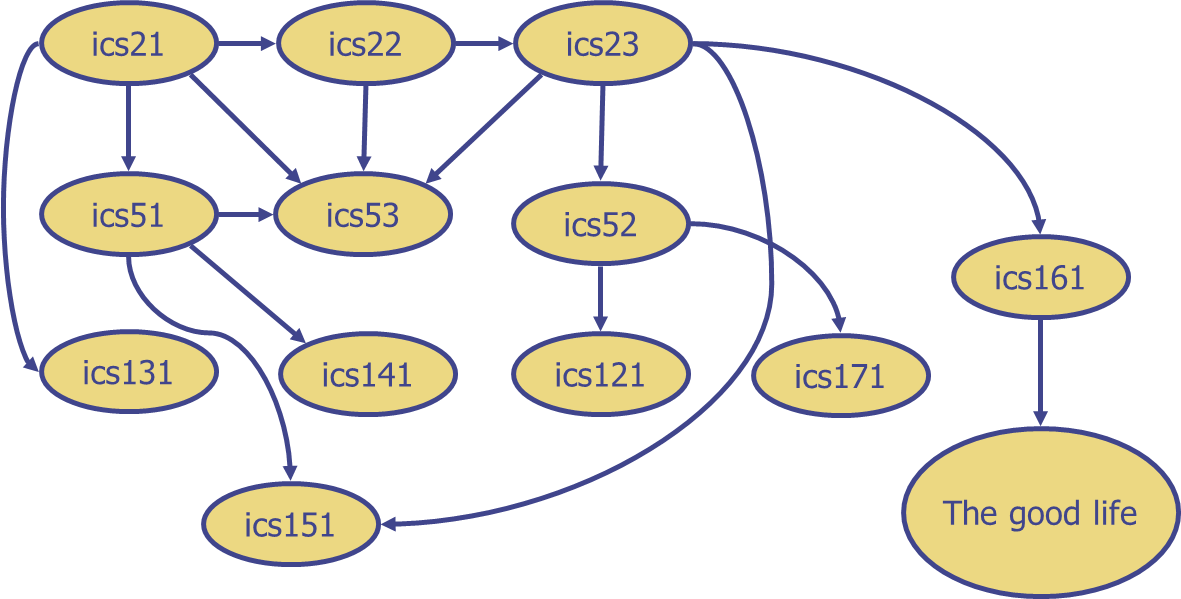
\includegraphics[width=10cm]{asp-14-pic29.png}
  \end{center}
\end{frame}

\begin{frame}[fragile]
  \frametitle{DFS za usmereni graf}
  \begin{columns}
    \begin{column}[t]{6cm}
      \begin{itemize}
        \item biće četiri vrste grana:
        \begin{itemize}
          \item discovery
          \item back
          \item forward: vodi prema potomku u pokrivajućem stablu
          \item cross: vodi prema čvoru u pokrivajućem stablu koji nije ni predak ni potomak
        \end{itemize}
        \item DFS za usmereni graf polazeći od čvora $s$ određuje
          čvorove \myred{dostupne} iz $s$ 
      \end{itemize}
    \end{column}
    \begin{column}[t]{6cm}
      \begin{center}
        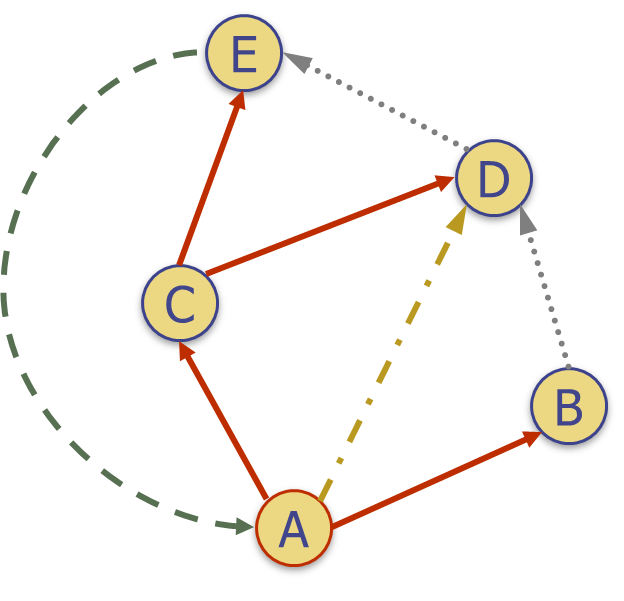
\includegraphics[width=5cm]{asp-14-pic30.png}
      \end{center}
    \end{column}
  \end{columns}
\end{frame}

\begin{frame}[fragile]
  \frametitle{Dostupnost}
  \begin{itemize}
    \item DFS \myred{stablo} sa korenom u $v$: čvorovi dostupni iz $v$
      duž usmerenih grana 
  \end{itemize}
  \begin{center}
    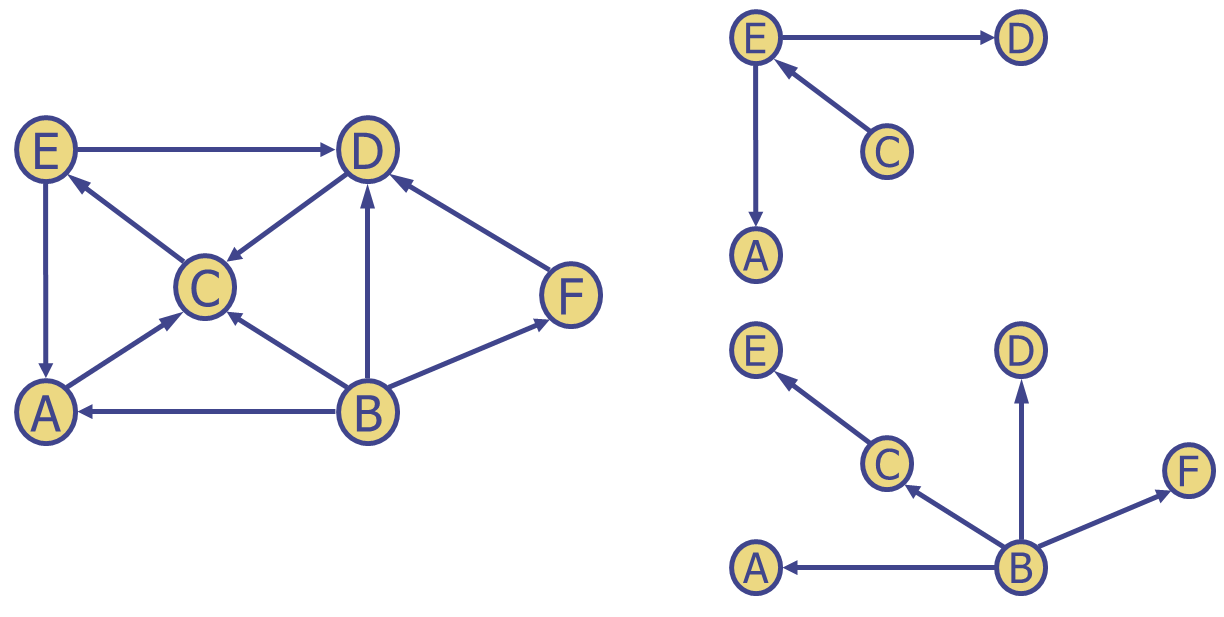
\includegraphics[width=10cm]{asp-14-pic31.png}
  \end{center}
\end{frame}

\begin{frame}[fragile]
  \frametitle{Jaka povezanost}
  \begin{itemize}
    \item iz svakog čvora se može stići do svakog drugog čvora
  \end{itemize}
  \begin{center}
    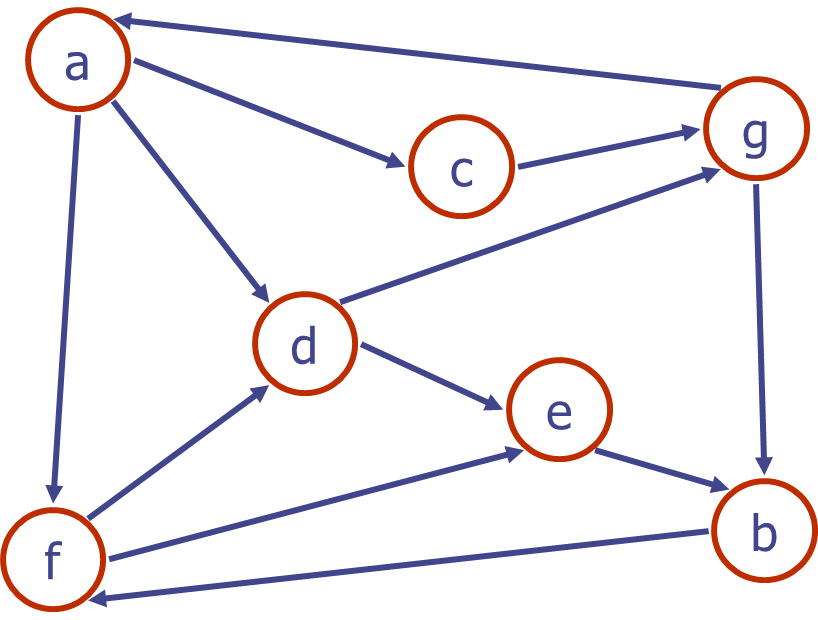
\includegraphics[width=6cm]{asp-14-pic32.png}
  \end{center}
\end{frame}

\begin{frame}[fragile]
  \frametitle{Jaka povezanost: algoritam}
  \begin{columns}
    \begin{column}[t]{6cm}
      \begin{itemize}
        \item izaberi čvor $v$ iz $G$
        \item uradi DFS iz $v$
        \begin{itemize}
          \item ako postoji $w$ koji nije obiđen, ispiši ,,ne``
        \end{itemize}
        \item neka je $G'$ dobijen okretanjem grana u $G$
        \item uradi DFS iz $v$ u $G'$
        \begin{itemize}
          \item ako postoji $w$ koji nije obiđen, ispiši ,,ne``
          \item inače ispiši ,,da``
        \end{itemize}
        \item vreme izvršavanja: $O(n+m)$
      \end{itemize}
    \end{column}
    \begin{column}[t]{6cm}
      \begin{center}
        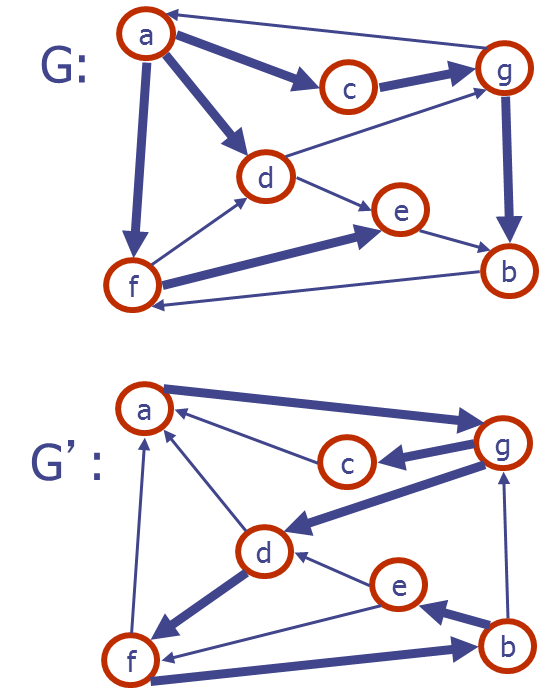
\includegraphics[width=5cm]{asp-14-pic33.png}
      \end{center}
    \end{column}
  \end{columns}
\end{frame}

\begin{frame}[fragile]
  \frametitle{Jako povezana komponenta}
  \begin{itemize}
    \item maksimalni podgraf takav da su iz svakog čvora dostupni svi
      drugi čvorovi
    \item takođe traje $O(n+m)$ pomoću DFS ali je složenije
  \end{itemize}
  \begin{center}
    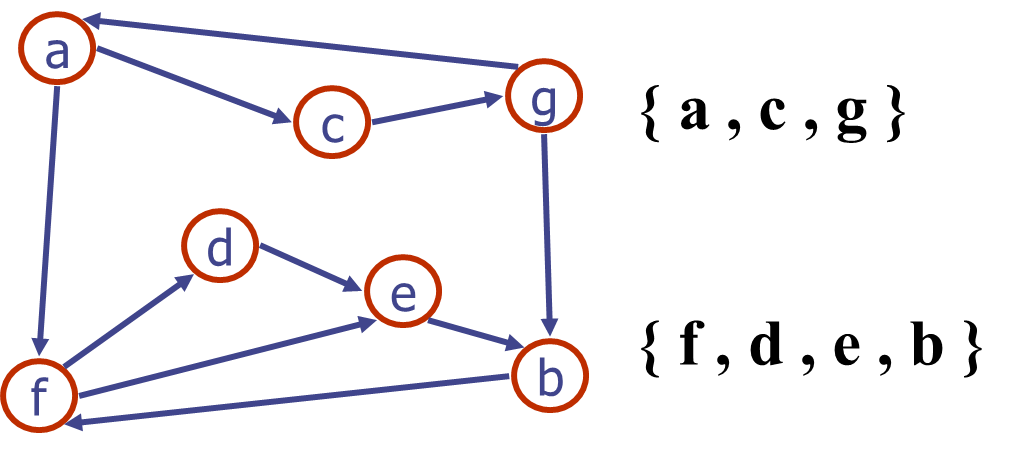
\includegraphics[width=8cm]{asp-14-pic34.png}
  \end{center}
\end{frame}

\begin{frame}[fragile]
  \frametitle{Tranzitivno zatvorenje}
  \begin{columns}
    \begin{column}[t]{6cm}
      \begin{itemize}
        \item za dati usmereni graf $G$, \myred{tranzitivno zatvorenje} 
          od $G$ je usmereni graf $G^{*}$ takav da
        \begin{itemize}
          \item $G^{*}$ ima iste čvorove kao $G$
          \item ako $G$ ima putanju od $u$ do $v$ ($u\neq v$), $G^{*}$ 
            ima granu od $u$ do $v$
        \end{itemize}
        \item tranzitivno zatvorenje daje informaciju o dostupnosti
          unutar usmerenog grafa
      \end{itemize}
    \end{column}
    \begin{column}[t]{6cm}
      \begin{center}
        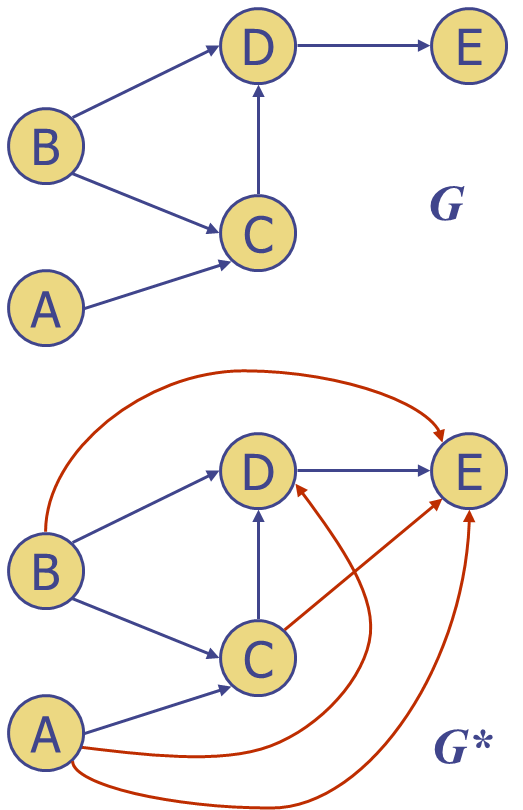
\includegraphics[width=4cm]{asp-14-pic35.png}
      \end{center}
    \end{column}
  \end{columns}
\end{frame}

\begin{frame}[fragile]
  \frametitle{Izračunavanje tranzitivnog zatvorenja}
  \begin{itemize}
    \item možemo raditi DFS iz svakog čvora -- traje $O(n(n+m))$
    \item možemo koristiti dinamičko programiranje -- Floyd-Warshall 
      algoritam
  \end{itemize}
\end{frame}

\begin{frame}[fragile]
  \frametitle{Floyd-Warshall algoritam}
  \begin{itemize}
    \item ideja \#1: označi čvorove brojevima $1, 2, \ldots, n$
    \item ideja \#2: razmatramo putanje koje imaju samo čvorove $1, 2, 
      \ldots, k$ kao međučvorove
  \end{itemize}
  \begin{center}
    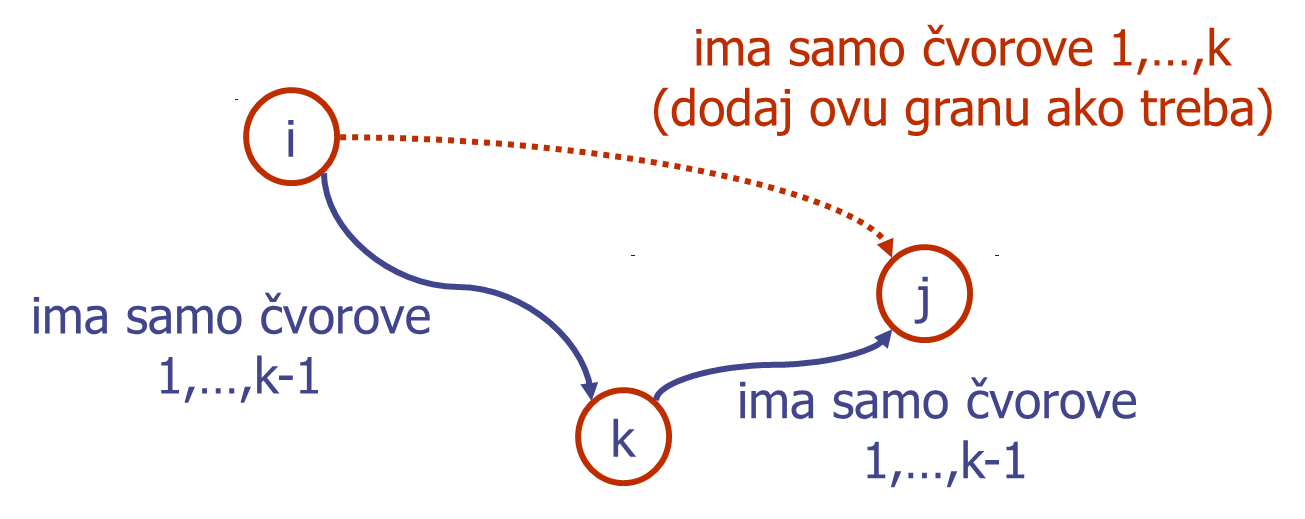
\includegraphics[width=10cm]{asp-14-pic36.png}
  \end{center}
\end{frame}

\begin{frame}[fragile]
  \frametitle{Floyd-Warshall algoritam}
  \begin{itemize}
    \item numeriši čvorove $v_1 \ldots v_n$
    \item izračunaj grafove $G_0 \ldots G_n$ 
    \begin{itemize}
      \item $G_0 = G$
      \item $G_k$ ima granu $(v_{i},v_{j})$ ako $G$ ima putanju 
        $v_{i}\rightarrow v_{j}$ sa međučvorovima u $\{v_{1}\ldots 
        v_{k}\}$
    \end{itemize}
    \item na kraju će biti $G_{n} = G^{*}$
    \item u fazi $k$, $G_{k}$ se računa iz $G_{k-1}$
    \item vreme je $O(n^3)$ ako \texttt{areAdjacent} je $O(1)$
      (koristi se matrica incidencije)
  \end{itemize}
\end{frame}

\begin{frame}[fragile,shrink=10]
  \frametitle{Floyd-Warshall algoritam}
  \begin{algorithmic}
    \STATE \myred{FloydWarshall}($G$)
    \STATE $i \leftarrow 1$
    \FORALL{$v \in G$.vertices()}
      \STATE označi $v$ kao $v_{i}$
      \STATE $i \leftarrow i+1$
    \ENDFOR
    \STATE $G_{0} \leftarrow G$
    \FOR{$k \leftarrow 1$ \TO $n$}
      \STATE $G_{k} \leftarrow G_{k-1}$
      \FOR{$i \leftarrow 1$ \TO $n (i \neq k)$}
        \FOR{$j \leftarrow 1$ \TO $n (j \neq i,k)$}
          \IF{$G_{k-1}$.areAdjacent($v_{i},v_{k}$) $\land G_{k-1}$.areAdjacent($v_{k},v_{j}$)}
            \IF{$\neg G_{k-1}$.areAdjacent($v_{i},v_{j}$)}
              \STATE $G_{k}$.insertEdge($v_{i},v_{j},k$)
            \ENDIF
          \ENDIF
        \ENDFOR
      \ENDFOR
    \ENDFOR
    \RETURN $G_{n}$
  \end{algorithmic}
\end{frame}

\begin{frame}[fragile,shrink=23]
  \frametitle{Floyd-Warshall u Pythonu}
\begin{minted}[linenos=false]{python}
def floyd_warshall(g):
  """Return a new graph that is the transitive closure of g."""
  closure = deepcopy(g)
  verts = list(closure.vertices())  # make indexable list
  n = len(verts)
  for k in range(n):
    for i in range(n):
      # verify that edge (i,k) exists in the partial closure
      if i != k and closure.get_edge(verts[i],verts[k]) is not None:
        for j in range(n):
          # verify that edge (k,j) exists in the partial closure
          if i != j != k and closure.get_edge(verts[k],verts[j]) is not None:
            # if (i,j) not yet included, add it to the closure
            if closure.get_edge(verts[i],verts[j]) is None:
              closure.insert_edge(verts[i],verts[j])
  return closure
\end{minted}
\end{frame}

\begin{frame}[fragile]
  \frametitle{Floyd-Warshall primer: $G_0$}
  \begin{center}
    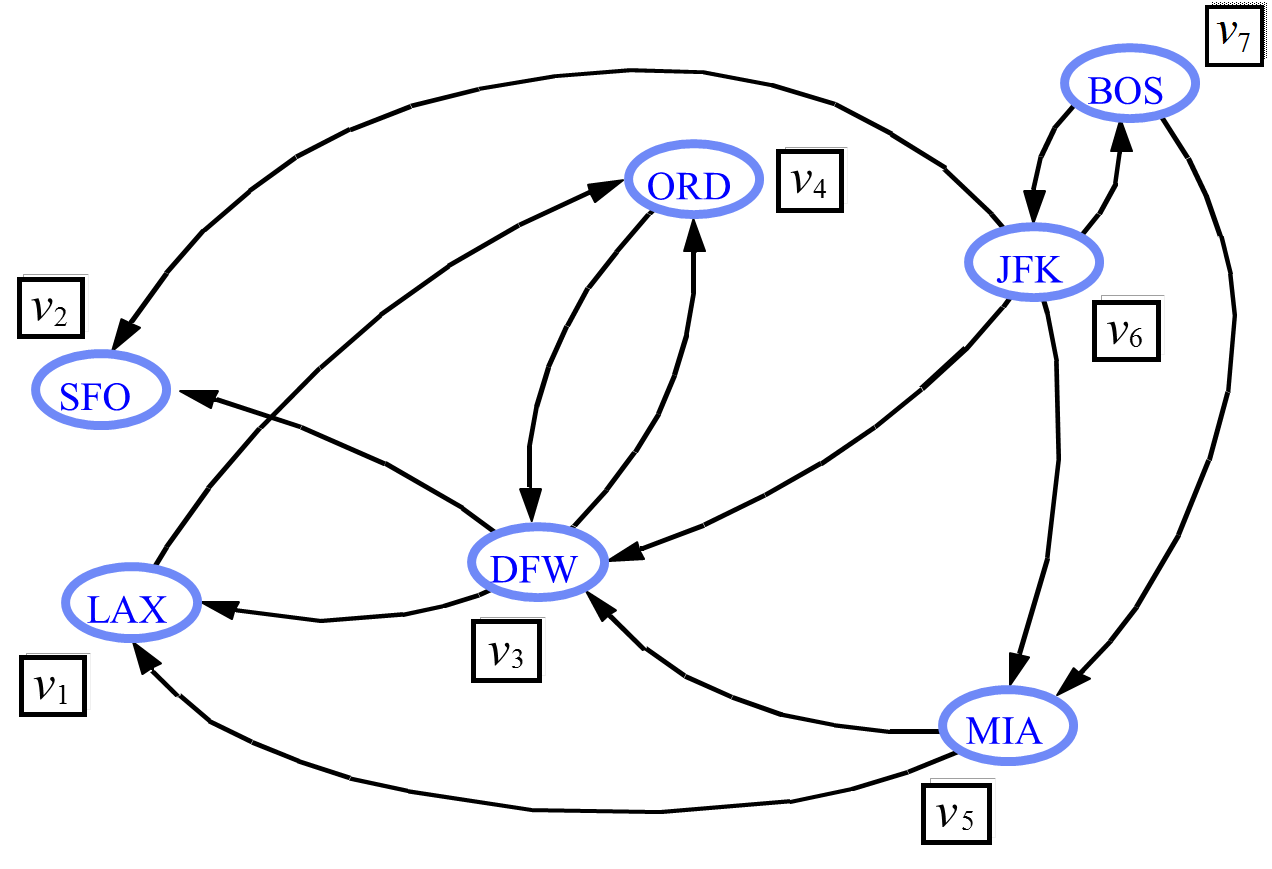
\includegraphics[width=10cm]{asp-14-pic37.png}
  \end{center}
\end{frame}

\begin{frame}[fragile]
  \frametitle{Floyd-Warshall primer: $G_1$}
  \begin{center}
    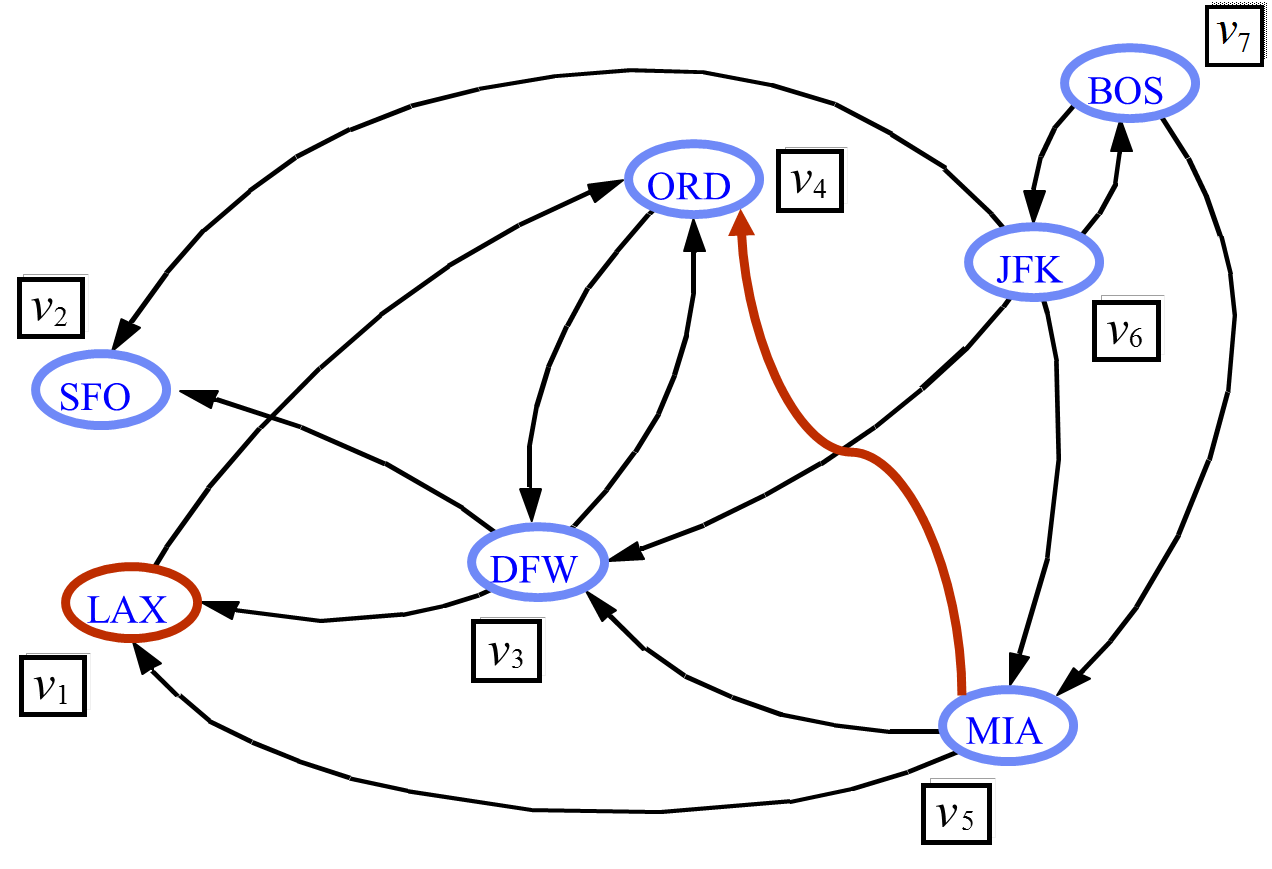
\includegraphics[width=10cm]{asp-14-pic38.png}
  \end{center}
\end{frame}

\begin{frame}[fragile]
  \frametitle{Floyd-Warshall primer: $G_2$}
  \begin{center}
    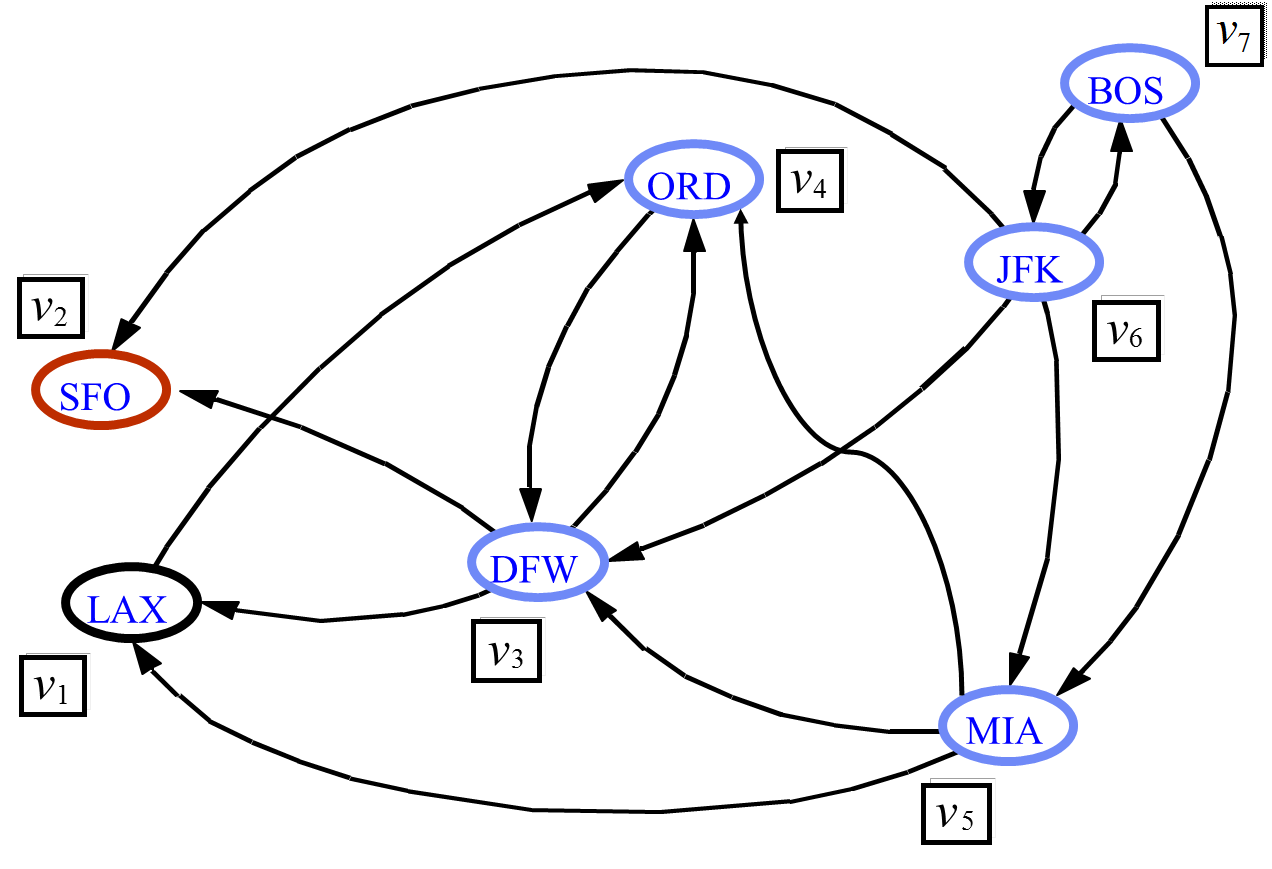
\includegraphics[width=10cm]{asp-14-pic39.png}
  \end{center}
\end{frame}

\begin{frame}[fragile]
  \frametitle{Floyd-Warshall primer: $G_3$}
  \begin{center}
    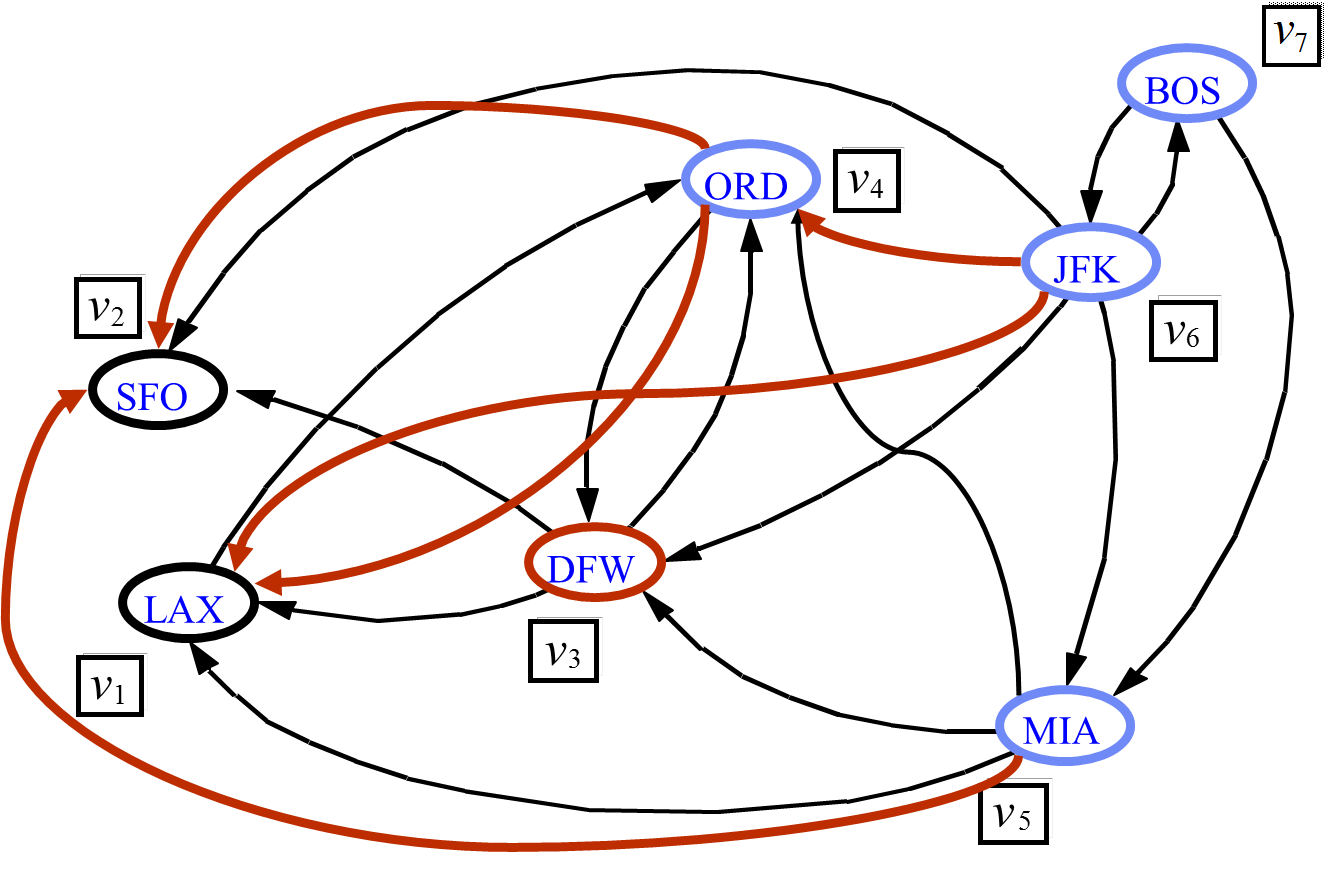
\includegraphics[width=10cm]{asp-14-pic40.png}
  \end{center}
\end{frame}

\begin{frame}[fragile]
  \frametitle{Floyd-Warshall primer: $G_4$}
  \begin{center}
    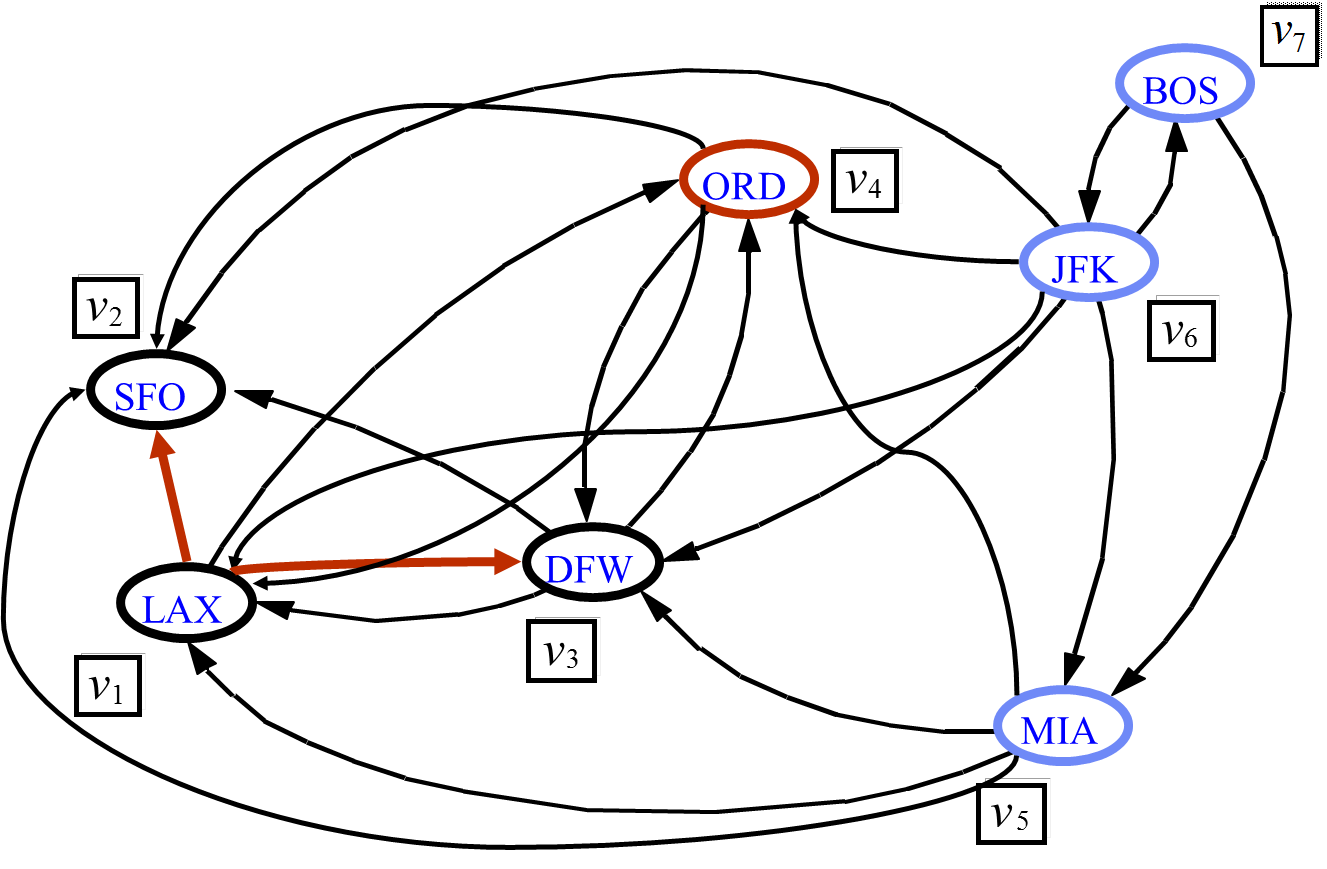
\includegraphics[width=10cm]{asp-14-pic41.png}
  \end{center}
\end{frame}

\begin{frame}[fragile]
  \frametitle{Floyd-Warshall primer: $G_5$}
  \begin{center}
    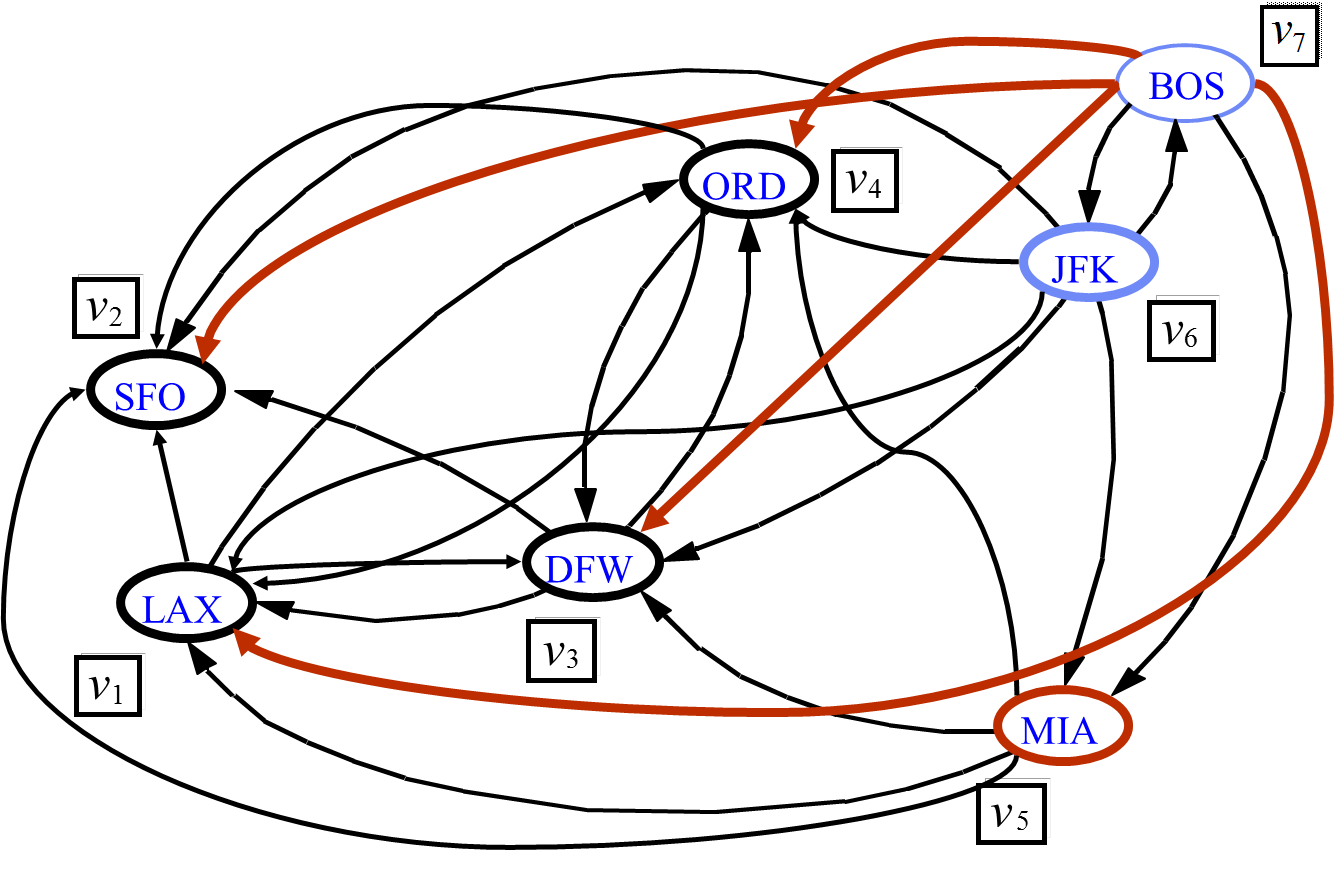
\includegraphics[width=10cm]{asp-14-pic42.png}
  \end{center}
\end{frame}

\begin{frame}[fragile]
  \frametitle{Floyd-Warshall primer: $G_6$}
  \begin{center}
    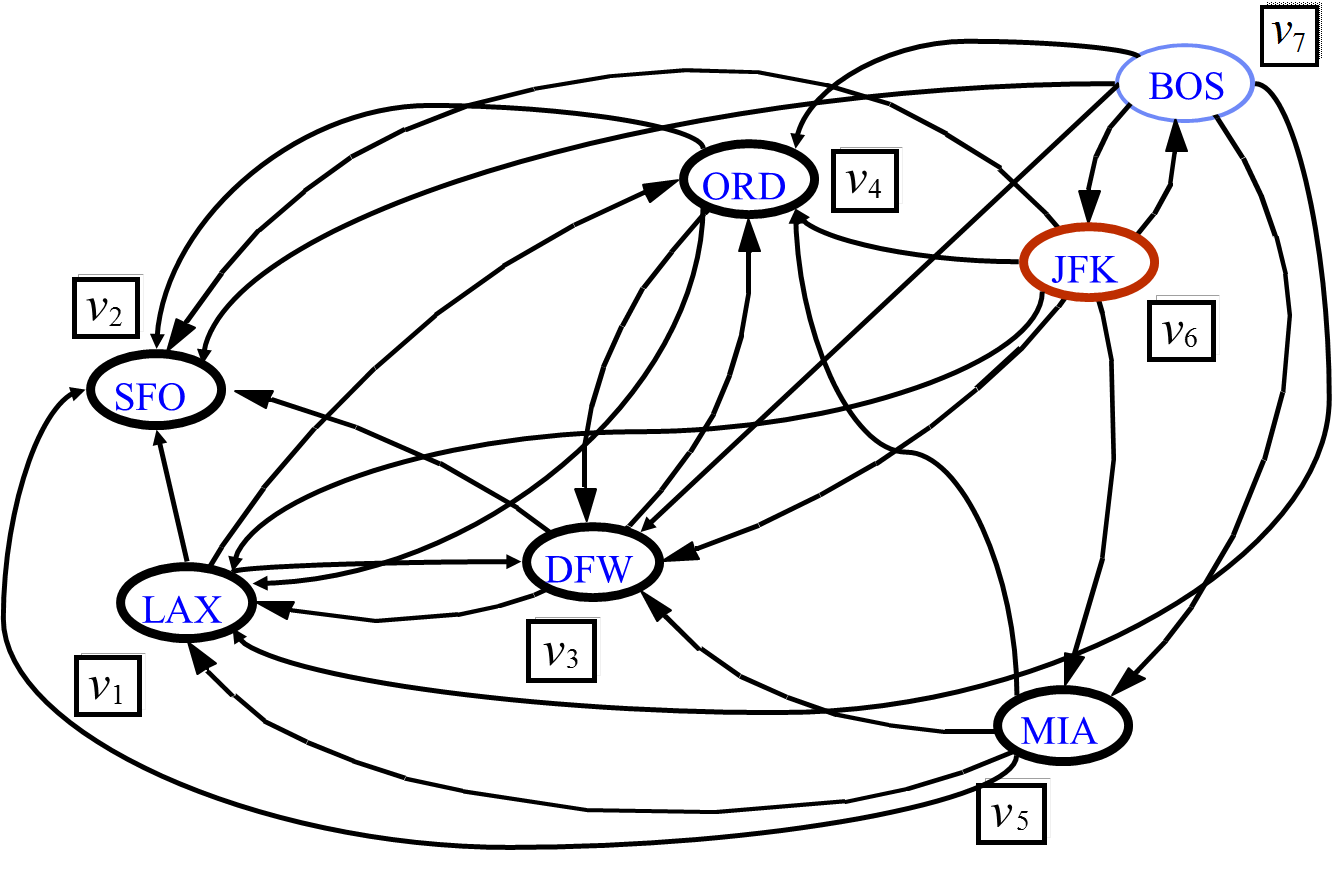
\includegraphics[width=10cm]{asp-14-pic43.png}
  \end{center}
\end{frame}

\begin{frame}[fragile]
  \frametitle{Floyd-Warshall primer: $G_7$}
  \begin{center}
    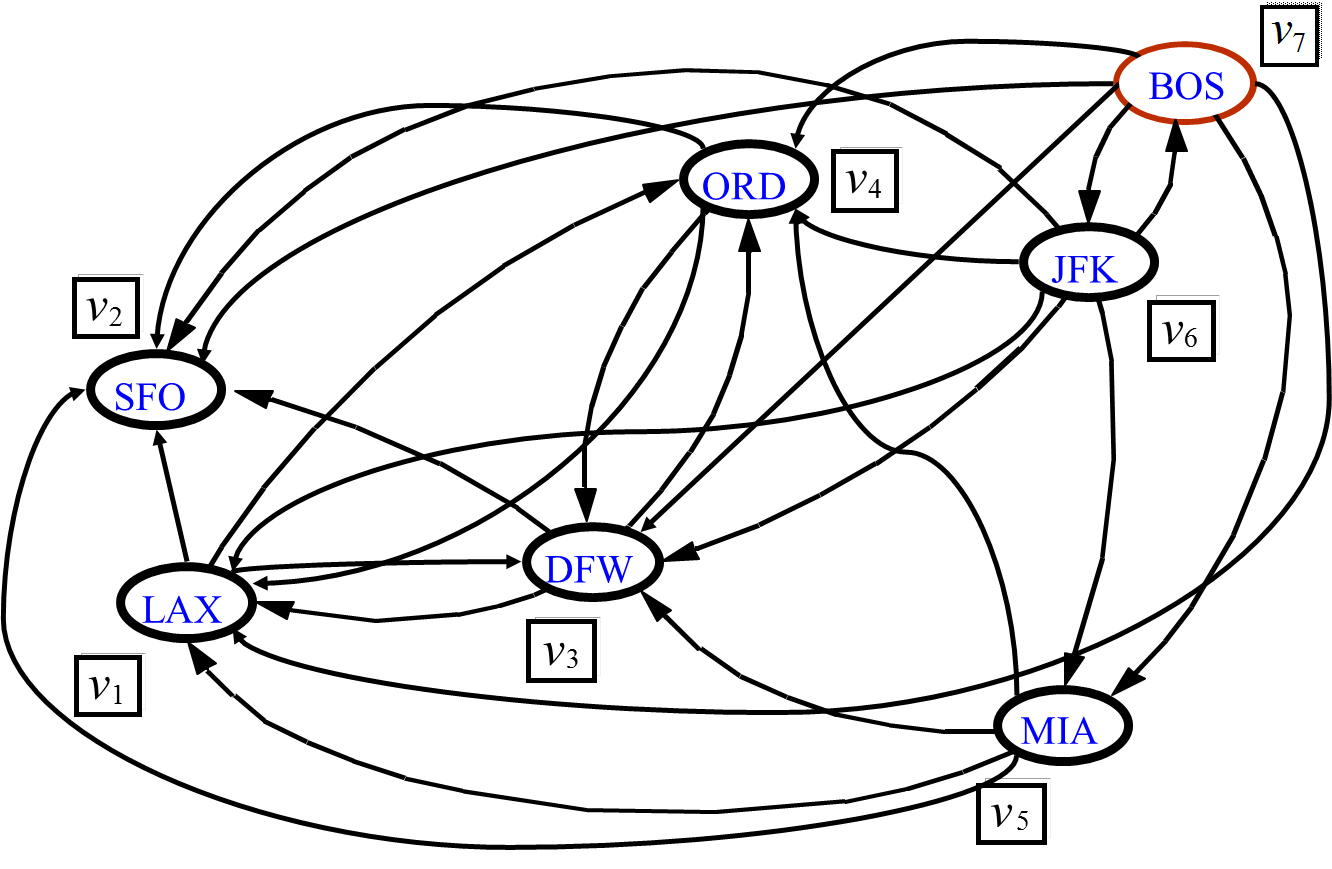
\includegraphics[width=10cm]{asp-14-pic44.png}
  \end{center}
\end{frame}

\begin{frame}[fragile]
  \frametitle{Topološko uređenje usmerenog grafa}
  \begin{columns}
    \begin{column}[t]{6cm}
      \begin{itemize}
        \item \myred{usmereni aciklični graf} (DAG) je aciklični graf 
          koji nema petlje
        \item topološko uređenje je numerisanje $v_{1} \ldots v_{n}$
          takvo da za svaku granu $(v_{i},v_{j})$ važi $i<j$
        \item primer: u grafu raspodele zadataka topološko uređenje je
          sekvenca zadataka koji ispunjavaju uslove prethođenja
        \item usmereni graf ima topološko uređenje akko je acikličan
      \end{itemize}
    \end{column}
    \begin{column}[t]{6cm}
      \begin{center}
        \hfill DAG $G$ \\
        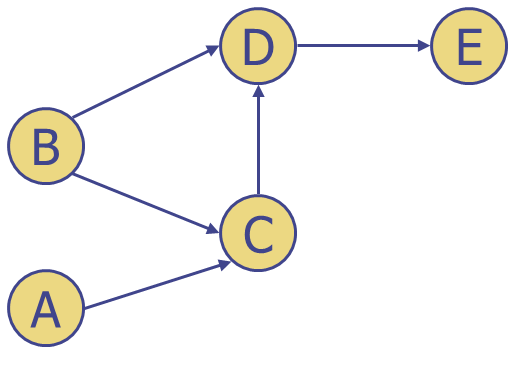
\includegraphics[width=3cm]{asp-14-pic45.png} \\ 
        \hfill topološko uređenje $G$ \\
        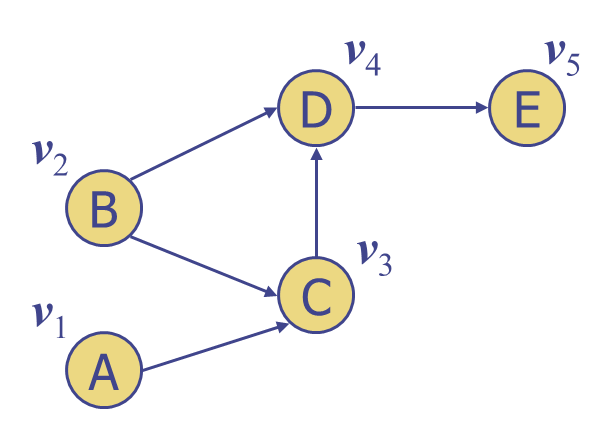
\includegraphics[width=3.5cm]{asp-14-pic46.png}
      \end{center}
    \end{column}
  \end{columns}
\end{frame}

\begin{frame}[fragile]
  \frametitle{Topološko sortiranje}
  \begin{itemize}
    \item numeriši čvorove tako da $(u,v) \in E$ implicira $u<v$ 
  \end{itemize}
  \begin{center}
    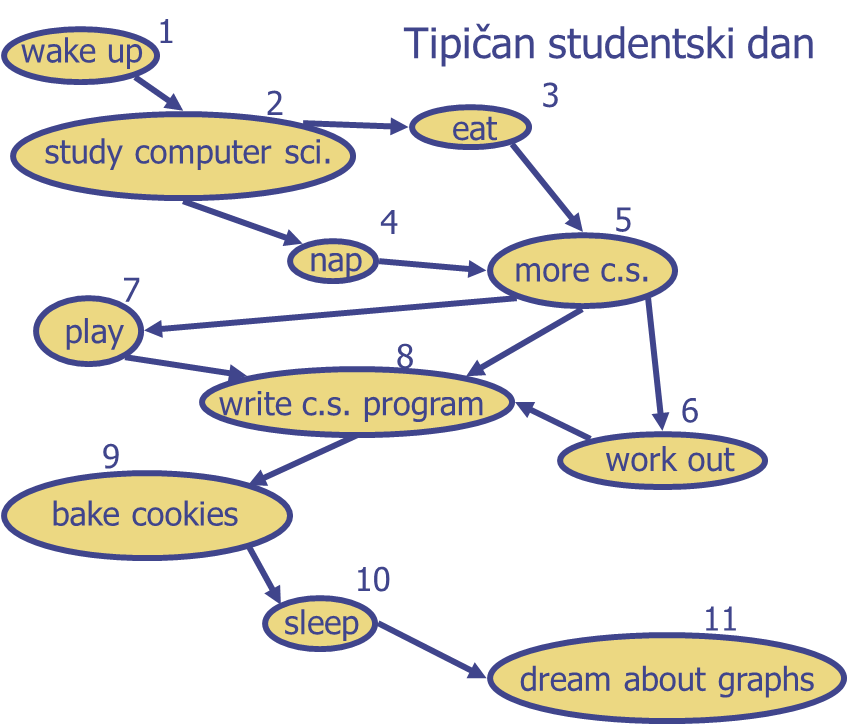
\includegraphics[width=7.4cm]{asp-14-pic47.png}
  \end{center}
\end{frame}

\begin{frame}[fragile]
  \frametitle{Algoritam za topološko sortiranje}
  \begin{algorithmic}
    \STATE \myred{TopologicalSort}($G$)
    \STATE $H \leftarrow G$.copy()
    \STATE $n \leftarrow G$.numVertices()
    \WHILE{$\neg H$.isEmpty()}
      \STATE $v$ je čvor bez izlaznih grana
      \STATE označi $v$ sa $n$
      \STATE $n \leftarrow n-1$
      \STATE $H$.remove($v$)
    \ENDWHILE
  \end{algorithmic}
  \hfill vreme je $O(n+m)$
\end{frame}

\renewcommand{\algorithmiccomment}[1]{\{\myred{#1}\}}

\begin{frame}[fragile]
  \frametitle{Topološko sortiranje pomoću DFS}
  {\small
  \begin{columns}
    \begin{column}[t]{6cm}
      \begin{algorithmic}
        \STATE \myred{topologicalDFS}($G$)
        \STATE $n \leftarrow G$.numVertices()
        \FORALL{$u\in G$.vertices()}
          \STATE setLabel($u$, {\scriptsize UNEXPLORED})
        \ENDFOR
        \FORALL{$v\in G$.vertices()}
          \IF{label($v$) = {\scriptsize UNEXPLORED}}
            \STATE topologicalDFS($G,v$)
          \ENDIF
        \ENDFOR
      \end{algorithmic}
    \end{column}
    \begin{column}[t]{6cm}
      \begin{algorithmic}
        \STATE \myred{topologicalDFS}($G,v$)
        \STATE setLabel($v$, {\scriptsize VISITED})
        \FORALL{$e \in G$.outEdges($v$)}
          \STATE $w \leftarrow$ opposite($v,e$)
          \IF{label($w$) = {\scriptsize UNEXPLORED}}
            \STATE \COMMENT{$e$ je {\scriptsize DISCOVERY}}
            \STATE topologicalDFS($G,w$) 
          \ELSE
            \STATE \COMMENT{$e$ je {\scriptsize FORWARD} ili {\scriptsize CROSS}}
            \STATE označi $v$ brojem $n$ 
          \ENDIF
        \ENDFOR{}
        \STATE $n \leftarrow n-1$
      \end{algorithmic}
    \end{column}
  \end{columns}
  }
\end{frame}

\begin{frame}[fragile]
  \frametitle{Topološko sortiranje: primer $_1$}
  \begin{center}
    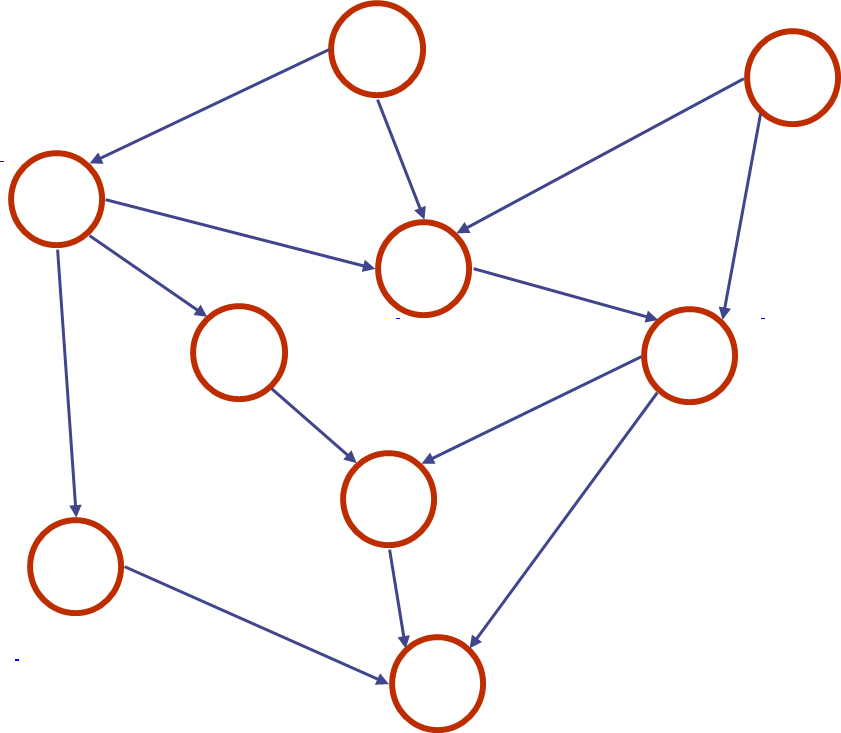
\includegraphics[width=7cm]{asp-14-pic48.png}
  \end{center}
\end{frame}

\begin{frame}[fragile]
  \frametitle{Topološko sortiranje: primer $_2$}
  \begin{center}
    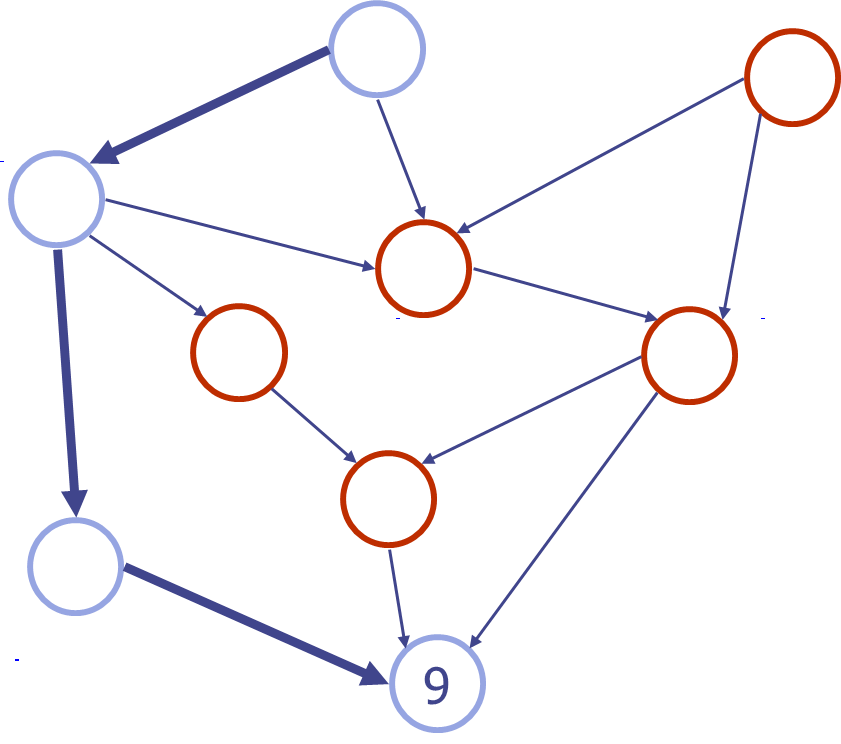
\includegraphics[width=7cm]{asp-14-pic49.png}
  \end{center}
\end{frame}

\begin{frame}[fragile]
  \frametitle{Topološko sortiranje: primer $_3$}
  \begin{center}
    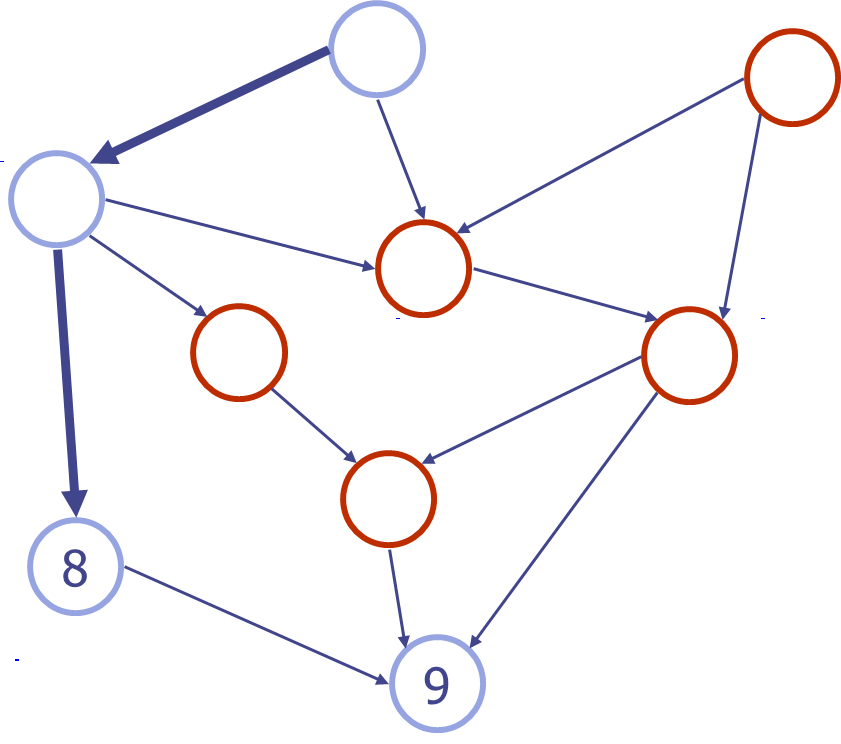
\includegraphics[width=7cm]{asp-14-pic50.png}
  \end{center}
\end{frame}

\begin{frame}[fragile]
  \frametitle{Topološko sortiranje: primer $_4$}
  \begin{center}
    \includegraphics[width=7cm]{asp-14-pic51.png}
  \end{center}
\end{frame}

\begin{frame}[fragile]
  \frametitle{Topološko sortiranje: primer $_5$}
  \begin{center}
    \includegraphics[width=7cm]{asp-14-pic52.png}
  \end{center}
\end{frame}

\begin{frame}[fragile]
  \frametitle{Topološko sortiranje: primer $_6$}
  \begin{center}
    \includegraphics[width=7cm]{asp-14-pic53.png}
  \end{center}
\end{frame}

\begin{frame}[fragile]
  \frametitle{Topološko sortiranje: primer $_7$}
  \begin{center}
    \includegraphics[width=7cm]{asp-14-pic54.png}
  \end{center}
\end{frame}

\begin{frame}[fragile]
  \frametitle{Topološko sortiranje: primer $_8$}
  \begin{center}
    \includegraphics[width=7cm]{asp-14-pic55.png}
  \end{center}
\end{frame}

\begin{frame}[fragile]
  \frametitle{Topološko sortiranje: primer $_9$}
  \begin{center}
    \includegraphics[width=7cm]{asp-14-pic56.png}
  \end{center}
\end{frame}

\begin{frame}[fragile]
  \frametitle{Topološko sortiranje: primer $_{10}$}
  \begin{center}
    \includegraphics[width=7cm]{asp-14-pic57.png}
  \end{center}
\end{frame}

\section[Težinski graf]{Težinski graf}

\begin{frame}[fragile]
  \frametitle{Težinski graf}
  \begin{itemize}
    \item svaka grana ima dodeljenu \myred{težinu}
    \item može da predstavlja rastojanje, trošak, itd.
    \item primer: rastojanje između aerodroma
  \end{itemize}
  \begin{center}
    \includegraphics[width=11cm]{asp-14-pic58.png}
  \end{center}
\end{frame}

\begin{frame}[fragile]
  \frametitle{Najkraći put}
  \begin{itemize}
    \item za dati težinski graf i čvorove $u$ i $v$ želimo da nađemo
      putanju sa najmanjom ukupnom težinom između $u$ i $v$
    \item težina putanje je suma težina grana u putanji
    \item primer: rutiranje paketa u mreži
  \end{itemize}
  \begin{center}
    \includegraphics[width=11cm]{asp-14-pic59.png}
  \end{center}
\end{frame}

\begin{frame}[fragile]
  \frametitle{Osobine najkraćeg puta}
  \begin{itemize}
    \item[1] podput najkraćeg puta je takođe najkraći put
    \item[2] postoji stablo najkraćih puteva od početnog čvora do svih
      ostalih čvorova
  \end{itemize}
  \begin{center}
    \includegraphics[width=11cm]{asp-14-pic60.png}
  \end{center}
\end{frame}

\begin{frame}[fragile]
  \frametitle{Dijkstra algoritam}
  \begin{columns}
    \begin{column}[t]{6cm}
      \begin{itemize}
        \item \myred{rastojanje} od čvora $v$ do čvora $s$ je dužina 
          najkraćeg puta $v \rightarrow s$
        \item Dajkstrin algoritam računa rastojanja do svih čvorova od
          datog čvora $s$
        \item pretpostavke:
        \begin{itemize}
          \item graf je povezan
          \item grane nisu usmerene
          \item težine nisu negativne
        \end{itemize}
      \end{itemize}
    \end{column}
    \begin{column}[t]{6cm}
      \begin{itemize}
        \item stvaramo ,,oblak`` čvorova počevši od $s$ dok ne uključimo
          sve čvorove
        \item za svaki čvor $v$ čuvamo labelu $d(v)$ koja predstavlja
          rastojanje od $v$ do $s$ u podgrafu sastavljenom od čvorova iz
          oblaka
        \item u svakom koraku:
        \begin{itemize}
          \item u oblak dodamo čvor $u$ sa najmanjim rastojanjem $d(u)$
          \item ažuriramo labele čvorova susednih sa $u$
        \end{itemize}
      \end{itemize}
    \end{column}
  \end{columns}
\end{frame}

\begin{frame}[fragile]
  \frametitle{Relaksiranje grana}
  \begin{columns}
    \begin{column}[t]{6cm}
      \begin{itemize}
        \item posmatramo granu $e=(u,z)$ takvu da
        \begin{itemize}
          \item $u$ je čvor poslednji dodat u oblak
          \item $z$ nije u oblaku
        \end{itemize}
        \item reklasiranje grane $e$ ažurira rastojanje $d(z)$:
          $$ d(z) \leftarrow \min\{d(z), d(u)+weight(e)\}$$
      \end{itemize}
    \end{column}
    \begin{column}[t]{6cm}
  \begin{center}
    \includegraphics[width=5cm]{asp-14-pic61.png}
  \end{center}
    \end{column}
  \end{columns}
\end{frame}

\begin{frame}[fragile]
  \frametitle{Dijkstra primer $_1$}
  \begin{center}
    \includegraphics[width=11cm]{asp-14-pic62.png}
  \end{center}
\end{frame}

\begin{frame}[fragile]
  \frametitle{Dijkstra primer $_2$}
  \begin{center}
    \includegraphics[width=11cm]{asp-14-pic63.png}
  \end{center}
\end{frame}

\begin{frame}[fragile]
  \frametitle{Dijkstra algoritam}
  \begin{algorithmic}
    \STATE \myred{ShortestPath}($G,s$)
    \STATE $D[s] \leftarrow 0$, $D[v]=\infty$ za svaki čvor $v\neq s$
    \STATE red sa prioritetom $Q$ sadrži sve čvorove iz $G$, ključevi su iz $D$
    \WHILE{$\neg Q$.isEmpty()}
      \STATE \COMMENT{dodaj novi čvor $u$ u oblak}
      \STATE $u \leftarrow Q$.removeMin() 
      \FORALL{$v\in Q$ koji je sused od $u$}
        \STATE \COMMENT{relaksiraj granu $(u,v)$}
        \IF{$D[u]+w(u,v)<D[v]$}
          \STATE $D[v] \leftarrow D[u]+w(u,v)$
          \STATE promeni ključ za $v$ na $D[v]$ u $Q$
        \ENDIF
      \ENDFOR
    \ENDWHILE
    \RETURN $D[v]$ za svaki čvor $v$
  \end{algorithmic}
\end{frame}

\begin{frame}[fragile]
  \frametitle{Dijkstra algoritam: analiza}
  \begin{itemize}
    \item operacije nad grafom
    \begin{itemize}
      \item nalazimo susedne grane po jednom za svaki čvor
    \end{itemize}
    \item operacije sa labelama
    \begin{itemize}
      \item za čvor $z$ postavljamo rastojanje i labele $O(deg(z))$ puta
      \item postavljanje labele traje $O(1)$
    \end{itemize}
    \item operacije nad redom sa prioritetom
    \begin{itemize}
      \item svaki čvor se dodaje jednom i uklanja jednom iz RSP, svaka 
        operacija traje $O(\log n)$
      \item ključ čvora u RSP se menja najviše $deg(w)$ puta, svaka 
        zamena ključa traje $O(\log n)$
      \item postavljanje labele traje $O(1)$
    \end{itemize}
    \item Dajkstrin algoritam traje $O((n+m)\log n)$ ako je u 
      implementaciji korišćena lista suseda
  \end{itemize}
\end{frame}

\begin{frame}[fragile,shrink]
  \frametitle{Python implementacija}
\begin{minted}[linenos=false]{python}
def shortest_path_lengths(g, src):
  d = {}                            # d[v] is upper bound from s to v
  cloud = {}                        # map reachable v to its d[v] value
  pq = AdaptableHeapPriorityQueue() # vertex v will have key d[v]
  pqlocator = {}                    # map from vertex to its pq locator

  # for each vertex v of the graph, add an entry to the priority queue, with
  # the source having distance 0 and all others having infinite distance
  for v in g.vertices():
    if v is src:
      d[v] = 0
    else:
      d[v] = float('inf')           # syntax for positive infinity
    pqlocator[v] = pq.add(d[v], v)  # save locator for future updates

  while not pq.is_empty():
    key, u = pq.remove_min()
    cloud[u] = key                  # its correct d[u] value
    del pqlocator[u]                # u is no longer in pq
    for e in g.incident_edges(u):   # outgoing edges (u,v)
      v = e.opposite(u)
      if v not in cloud:
        # perform relaxation step on edge (u,v)
        wgt = e.element()
        if d[u] + wgt < d[v]:       # better path to v?
          d[v] = d[u] + wgt         # update the distance
          pq.update(pqlocator[v], d[v], v) # update the pq entry

  return cloud                # only includes reachable vertices
\end{minted}
\end{frame}

\begin{frame}[fragile]
  \frametitle{Dijkstra i pohlepa}
  \begin{columns}
    \begin{column}[t]{11cm}
      \begin{itemize}
        \item Dijkstra koristi pohlepni metod -- dodaje čvorove po 
          rastućem rastojanju
        \item pretpostavimo da nije našao najkraća rastojanja; neka je 
          $F$ prvi pogrešan čvor
        \item najkraći put je bio OK za prethodni čvor $D$
        \item ali grana $(D,F)$ je tada relaksirana
        \item prema tome, sve dok je $d(F)\geq d(D)$, $d(F)$ nije
          pogrešno, tj. nismo pogrešili čvor
      \end{itemize}
    \end{column}
    \begin{column}[t]{5cm}
      \begin{center}
        \includegraphics[width=5cm]{asp-14-pic64.png}
      \end{center}
    \end{column}
  \end{columns}
\end{frame}

\begin{frame}[fragile]
  \frametitle{Dijkstra ne radi za negativne težine}
  \begin{columns}
    \begin{column}[t]{7cm}
      \begin{itemize}
        \item Dijkstra koristi pohlepni metod -- dodaje čvorove po 
          rastućem rastojanju
        \item ako bi čvor sa negativnom granom bio dodat u oblak,
          pokvario bi rastojanja čvorova koji su već tamo
      \end{itemize}
    \end{column}
    \begin{column}[t]{5cm}
      \begin{center}
        \includegraphics[width=5cm]{asp-14-pic65.png}
      \end{center}
    \end{column}
  \end{columns}
\end{frame}

\begin{frame}[fragile,shrink=2]
  \frametitle{Bellman-Ford algoritam}
  \begin{columns}
    \begin{column}[t]{7cm}
      \begin{itemize}
        \item radi i za negativne težine
        \item grane moraju biti usmerene -- inače bismo imali negativne 
          petlje!
        \item $i$-ta iteracija pronalazi najkraće puteve sa $i$ grana
        \item vreme: $O(nm)$
      \end{itemize}
    \end{column}
    \begin{column}[t]{7cm}
      \begin{algorithmic}
        \STATE \myred{BellmanFord}($G,s$)
        \FORALL{$v \in G$.vertices()}
          \IF{$v = s$}
            \STATE setDistance($v,0$)
          \ELSE
            \STATE setDistance($v,\infty$)
          \ENDIF
        \ENDFOR
        \FOR{$i \leftarrow 1$ \TO $n-1$}
          \FORALL{$e \in G$.edges()}
            \STATE \COMMENT{relaksiraj granu $e$}
            \STATE $u \leftarrow G$.origin($e$)
            \STATE $z \leftarrow G$.opposite($u,e$)
            \STATE $r \leftarrow$ getDistance($u$) + weight($e$)
            \IF{$r < $getDistance($z$)}
              \STATE setDistance($z,r$)
            \ENDIF
          \ENDFOR
        \ENDFOR
      \end{algorithmic}
    \end{column}
  \end{columns}
\end{frame}

\begin{frame}[fragile]
  \frametitle{Bellman-Ford primer}
  \begin{center}
    \includegraphics[width=11cm]{asp-14-pic66.png}
  \end{center}
  \hfill {\scriptsize čvorovi su označeni sa $d(v)$}
\end{frame}

\begin{frame}[fragile,shrink=2]
  \frametitle{Algoritam za usmereni aciklični graf}
  \begin{columns}
    \begin{column}[t]{5cm}
      \begin{itemize}
        \item radi i za negativne težine
        \item koristi topološko uređenje
        \item ne koristi posebnu strukturu podataka
        \item znatno brži od Dijkstre: $O(n+m)$
      \end{itemize}
    \end{column}
    \begin{column}[t]{7cm}{\small
      \begin{algorithmic}
        \STATE \myred{DagDistances}($G,s$)
        \FORALL{$v \in G$.vertices()}
          \IF{$v = s$}
            \STATE setDistance($v,0$)
          \ELSE
            \STATE setDistance($v,\infty$)
          \ENDIF
        \ENDFOR
        \STATE \COMMENT{topološki sortiraj čvorove}
        \FOR{$u \leftarrow 1$ \TO $n$}
          \STATE \COMMENT{u topološkom redosledu}
          \FORALL{$e \in G$.outEdges($u$)}
            \STATE \COMMENT{relaksiraj granu $e$}
            \STATE $z \leftarrow G$.opposite($u,e$)
            \STATE $r \leftarrow$ getDistance($u$) + weight($e$)
            \IF{$r < $getDistance($z$)}
              \STATE setDistance($z,r$)
            \ENDIF
          \ENDFOR
        \ENDFOR
      \end{algorithmic}}
    \end{column}
  \end{columns}
\end{frame}

\begin{frame}[fragile]
  \frametitle{DAG primer}
  \begin{center}
    \includegraphics[width=11cm]{asp-14-pic67.png}
  \end{center}
  \hfill {\scriptsize čvorovi su označeni sa $d(v)$}
\end{frame}

\section[Minimalno pokrivajuće stablo]{Minimalno pokrivajuće stablo}

\begin{frame}[fragile]
  \frametitle{Minimalno pokrivajuće stablo}
  \begin{columns}
    \begin{column}[t]{7cm}
      \begin{itemize}
        \item \myred{pokrivajući podgraf}: podgraf od $G$ koji sadrži 
          sve čvorove iz $G$
        \item \myred{pokrivajuće stablo}: pokrivajući podgraf koji je
          stablo
        \item \myred{minimalno pokrivajuće stablo}: pokrivajuće stablo
          sa najmanjom sumom težina grana
        \item ,,minimum spanning tree`` (MST)
      \end{itemize}
    \end{column}
    \begin{column}[t]{5cm}
      \begin{center}
        \includegraphics[width=5cm]{asp-14-pic68.png}
      \end{center}
    \end{column}
  \end{columns}
\end{frame}

\begin{frame}[fragile]
  \frametitle{MST i petlje}
  \begin{columns}
    \begin{column}[t]{7cm}
      \begin{itemize}
        \item $T$ je MST grafa $G$
        \item $e$ je grana koja nije u $T$
        \item $C$ je petlja koju $e$ pravi sa $T$
        \item za svaku granu $f$ iz $C$ važi: \\ $weight(f)\leq weight(e)$
        \item dokaz kontradikcijom: ako bi bilo $weight(f)>weight(e)$
          imali bismo MST sa manjom težinom zamenom $e$ sa $f$
      \end{itemize}
    \end{column}
    \begin{column}[t]{5cm}
      \begin{center}
        \includegraphics[width=4.5cm]{asp-14-pic70.png}
      \end{center}
    \end{column}
  \end{columns}
\end{frame}

\begin{frame}[fragile]
  \frametitle{MST i particije}
  \begin{columns}
    \begin{column}[t]{7cm}
      \begin{itemize}
        \item posmatramo podelu čvorova iz $G$ na podskupove $U$ i $V$
        \item $e$ je grana između podskupova sa najmanjom težinom
        \item postoji MST od $G$ koji sadrži $e$
        \item dokaz: $T$ je MST od $G$
        \item ako $T$ ne sadrži $e$, posmatramo petlju $C$ koju čine $T$
          i $e$ i neka je $f$ grana iz $C$ koja prelazi particiju
        \item (prethodni slajd): $weight(f)\leq weight(e)$
        \item prema tome: $weight(f)=weight(e)$
        \item dobijamo novo MST zamenom $f$ sa $e$
      \end{itemize}
    \end{column}
    \begin{column}[t]{5cm}
      \begin{center}
        \includegraphics[width=4.3cm]{asp-14-pic71.png}
      \end{center}
    \end{column}
  \end{columns}
\end{frame}

\begin{frame}[fragile]
  \frametitle{Prim-Jarnik algoritam}
  \begin{itemize}
    \item sličan Dijkstra algoritmu
    \item izaberemo čvor $s$ i pravimo MST kao oblak čvorova počevši od 
      $s$
    \item čvor $v$ čuva labelu $d(v)$ -- najmanja težina grane koja
      povezuje $v$ sa oblakom
    \item u svakom koraku:
    \begin{itemize}
      \item dodamo u oblak čvor $u$ sa najmanjim $d(u)$
      \item ažuriramo labele čvorova susednih sa $u$
    \end{itemize}
  \end{itemize}
\end{frame}

\begin{frame}[fragile,shrink=2]
  \frametitle{Prim-Jarnik algoritam}
  \begin{algorithmic}
    \STATE \myred{PrimJarnik}($G$)
    \STATE izaberi bilo koji $s$ iz $G$
    \STATE $D[s] \leftarrow 0$
    \FORALL{čvor $v \neq s$}
      \STATE $D[v] \leftarrow \infty$
    \ENDFOR
    \STATE $T \leftarrow \emptyset$
    \STATE napuni RSP $Q$ elementima ($D[v]$,($v$,None)) za svaki čvor $v$
    \WHILE{$\neg Q$.isEmpty()}
      \STATE $(u,e) \leftarrow Q$.removeMin()
      \STATE poveži $u$ sa $T$ preko $e$
      \FORALL{$e'=(u,v) | v \in Q$}
        \STATE \COMMENT{da li $(u,v)$ bolje povezuje $v$ sa $T$}
        \IF{$w(u,v)<D[v]$}
          \STATE $D[v] \leftarrow w(u,v)$
          \STATE promeni ključ za $v$ u $Q$ na $D[v]$
          \STATE promeni vrednost za $v$ u $Q$ na ($v,e'$)
        \ENDIF
      \ENDFOR
    \ENDWHILE
    \RETURN $T$
  \end{algorithmic}
\end{frame}

\begin{frame}[fragile]
  \frametitle{Prim-Jarnik primer $_1$}
  \begin{center}
    \includegraphics[width=11cm]{asp-14-pic72.png}
  \end{center}
\end{frame}

\begin{frame}[fragile]
  \frametitle{Prim-Jarnik primer $_2$}
  \begin{center}
    \includegraphics[width=11cm]{asp-14-pic73.png}
  \end{center}
\end{frame}

\begin{frame}[fragile]
  \frametitle{Prim-Jarnik algoritam: analiza}
  \begin{itemize}
    \item operacije nad grafom
    \begin{itemize}
      \item prolazimo kroz susedne grane po jednom za svaki čvor
    \end{itemize}
    \item operacije sa labelama
    \begin{itemize}
      \item za čvor $z$ postavljamo rastojanje i labele $O(deg(z))$ puta
      \item postavljanje labele traje $O(1)$
    \end{itemize}
    \item operacije nad redom sa prioritetom
    \begin{itemize}
      \item svaki čvor se dodaje jednom i uklanja jednom iz RSP, svaka 
        operacija traje $O(\log n)$
      \item ključ čvora u RSP se menja najviše $deg(w)$ puta, svaka 
        zamena ključa traje $O(\log n)$
      \item postavljanje labele traje $O(1)$
    \end{itemize}
    \item Prim-Jarnik algoritam traje $O((n+m)\log n)$ ako je u 
      implementaciji korišćena lista suseda
  \end{itemize}
\end{frame}

\begin{frame}[fragile,shrink]
  \frametitle{Prim-Jarnik u Pythonu}
\begin{minted}[linenos=false]{python}
def MST_PrimJarnik(g):
  d = {}                            # d[v] is bound on distance to tree
  tree = []                         # list of edges in spanning tree
  pq = AdaptableHeapPriorityQueue() # d[v] maps to value (v, e=(u,v))
  pqlocator = {}                    # map from vertex to its pq locator

  # for each vertex v of the graph, add an entry to the priority queue, with
  # the source having distance 0 and all others having infinite distance
  for v in g.vertices():
    if len(d) == 0:                 # this is the first node
      d[v] = 0                      # make it the root
    else:
      d[v] = float('inf')           # positive infinity
    pqlocator[v] = pq.add(d[v], (v,None))

  while not pq.is_empty():
    key,value = pq.remove_min()
    u,edge = value                  # unpack tuple from pq
    del pqlocator[u]                # u is no longer in pq
    if edge is not None:
      tree.append(edge)             # add edge to tree
    for link in g.incident_edges(u):
      v = link.opposite(u)
      if v in pqlocator:            # thus v not yet in tree
        # see if edge (u,v) better connects v to the growing tree
        wgt = link.element()
        if wgt < d[v]:              # better edge to v?
          d[v] = wgt                # update the distance
          pq.update(pqlocator[v], d[v], (v, link)) # update the pq entry

  return tree
\end{minted}
\end{frame}

\begin{frame}[fragile]
  \frametitle{Kruskal algoritam}
  \begin{itemize}
    \item particija čvorova u klastere (grozdove)
    \begin{itemize}
      \item inicijalno klasteri sa po jednim čvorom
      \item održava se MST za svaki klaster
      \item spajanje ,,najbližih`` klastera i njihovih MST
    \end{itemize}
    \item red sa prioritetom čuva grane izvan klastera
    \begin{itemize}
      \item ključ: težina
      \item vrednost: grana
    \end{itemize}
    \item na kraju rada algoritma: jedan klaster i jedno MST
  \end{itemize}
\end{frame}

\begin{frame}[fragile,shrink=2]
  \frametitle{Kruskal algoritam}
  \begin{algorithmic}
    \STATE \myred{Kruskal}($G$)
    \FORALL{$v \in G$}
      \STATE postavi osnovni klaster $C(v) = \{v\}$
    \ENDFOR
    \STATE napuni RSP $Q$ granama iz $G$ koristeći težine kao ključeve
    \STATE $T \leftarrow \emptyset$
    \WHILE{$T$ ima manje od $n-1$ grana}
      \STATE $(u,e) \leftarrow Q$.removeMin()
      \STATE $C(u)$ je klaster koji sadrži $u$
      \STATE $C(v)$ je klaster koji sadrži $v$
      \IF{$C(u) \neq C(v)$}
        \STATE dodaj granu $(u,v)$ u $T$
        \STATE spoj $C(u)$ i $C(v)$ u jedan klaster
      \ENDIF
    \ENDWHILE
    \RETURN $T$
  \end{algorithmic}
\end{frame}

\begin{frame}[fragile]
  \frametitle{Kruskal primer $_1$}
  \begin{center}
    \includegraphics[width=11cm]{asp-14-pic74.png}
  \end{center}
\end{frame}

\begin{frame}[fragile]
  \frametitle{Kruskal primer $_2$}
  \begin{center}
    \includegraphics[width=11cm]{asp-14-pic75.png}
  \end{center}
\end{frame}

\begin{frame}[fragile]
  \frametitle{Struktura podataka za Kruskal algoritam: particija}
  \begin{itemize}
    \item algoritam rukuje šumom stabala
    \item RSP daje grane u redosledu rastućih težina
    \item grana se prihvata ako spaja različita stabla
    \item potrebna je struktura podataka koja čuva \myred{particiju},
      tj. kolekciju disjunktnih skupova, sa operacijama
    \begin{itemize}
      \item \myred{makeSet}($u$): kreiraj skup koji sadrži $u$
      \item \myred{find}($u$): nađi skup koji sadrži $u$
      \item \myred{union}($A,B$): zameni skupove $A$ i $B$ njihovom 
        unijom
    \end{itemize}
  \end{itemize}
\end{frame}

\begin{frame}[fragile]
  \frametitle{Particija pomoću liste}
  \begin{itemize}
    \item svaki skup se čuva u sekvenci
    \item svaki element ima referencu na skup
    \begin{itemize}
      \item \myred{find}($u$) traje $O(1)$ i vraća skup koji sadrži $u$
      \item \myred{union}($A,B$): premeštamo elemente iz manjeg skupa u
        veći i ažuriramo reference na skup; traje $O(min\{|A|,|B|\})$
    \end{itemize}
    \item kada se element obradi, prelazi u skup koji je bar duplo veći,
      dakle svaki element se obrađuje najviše $\log n$ puta
  \end{itemize}
  \begin{center}
    \includegraphics[width=8cm]{asp-14-pic77.png}
  \end{center}
\end{frame}

\begin{frame}[fragile]
  \frametitle{Kruskal pomoću particije}
  \begin{itemize}
    \item spajanje klastera pomoću \myred{union}
    \item pronalaženje klastera pomoću \myred{find}
    \item brzina je $O((n+m)\log n)$
    \begin{itemize}
      \item operacije sa RSP: $O(m\log n)$
      \item union-find operacije: $O(n\log n)$
    \end{itemize}
  \end{itemize}
\end{frame}

\begin{frame}[fragile,shrink]
  \frametitle{Kruskal u Pythonu}
\begin{minted}[linenos=false]{python}
def MST_Kruskal(g):
  tree = []                # list of edges in spanning tree
  pq = HeapPriorityQueue() # entries are edges in G, with weights as key
  forest = Partition()     # keeps track of forest clusters
  position = {}            # map each node to its Partition entry

  for v in g.vertices():
    position[v] = forest.make_group(v)

  for e in g.edges():
    pq.add(e.element(), e) # edge's element is assumed to be its weight

  size = g.vertex_count()
  while len(tree) != size - 1 and not pq.is_empty():
    # tree not spanning and unprocessed edges remain
    weight,edge = pq.remove_min()
    u,v = edge.endpoints()
    a = forest.find(position[u])
    b = forest.find(position[v])
    if a != b:
      tree.append(edge)
      forest.union(a,b)

  return tree
\end{minted}
\end{frame}

\begin{frame}[t,fragile]{Particija pomoću stabla}
  \begin{itemize}
    \item čvor stabla čuva element i referencu na skup
    \item čvor $v$ čija referenca pokazuje na $v$ je istovremeno i skup
    \item svaki skup je stablo, njegov koren čuva referencu na sebe
    \item na primer, skupovi ,,1``, ,,2`` i ,,5``
  \end{itemize}
  \begin{center}
    \includegraphics[width=8cm]{asp-14-pic78.png}
  \end{center}
\end{frame}

\begin{frame}[t]{Particija pomoću stabla: union i find}
  \begin{columns}
    \column{7cm}
      \begin{itemize}
        \item \myred{union}: koren jednog stabla treba da pokazuje na
          koren drugog
        \item \myred{find}: prati reference do korena koji pokazuje na 
          samog sebe
      \end{itemize}
    \column{7cm}
      \begin{center}
        \includegraphics[width=4cm]{asp-14-pic79.png}
      \end{center}
  \end{columns}
\end{frame}

\begin{frame}[fragile]
  \frametitle{Recepti za union-find}
  \begin{columns}
    \begin{column}[t]{7cm}
      \begin{itemize}
        \item kada se radi union, neka koren manjeg stabla pokaže na
          koren većeg
        \item $O(n\log n)$ vreme za izvođenje $n$ union-find operacija
        \begin{itemize}
          \item svaki put kada pratimo referencu, idemo prema stablu
            koje je bar duplo veće od trenutnog
          \item prema tome, pratimo najviše $O(\log n)$ referenci za
            svaki find
        \end{itemize}
      \end{itemize}
    \end{column}
    \begin{column}[t]{5cm}
      \begin{center}
        \includegraphics[width=4.5cm]{asp-14-pic80.png}
      \end{center}
    \end{column}
  \end{columns}
\end{frame}

\begin{frame}[fragile]
  \frametitle{Recepti za union-find}
  \begin{itemize}
    \item \myred{kompresija putanje}: nakon find, neka sve reference
      čvorova koje smo upravo obišli pokazuju na koren
    \end{itemize}
  \begin{center}
    \includegraphics[width=8cm]{asp-14-pic81.png}
  \end{center}
\end{frame}

\begin{frame}[fragile,shrink]
  \frametitle{Particija u Pythonu $_1$}
\begin{minted}[linenos=false]{python}
class Partition:
  class Position:
    __slots__ = '_container', '_element', '_size', '_parent'

    def __init__(self, container, e):
      """Create a new position that is the leader of its own group."""
      self._container = container  # reference to Partition instance
      self._element = e
      self._size = 1
      self._parent = self          # convention for a group leader

    def element(self):
      """Return element stored at this position."""
      return self._element

  def _validate(self, p):
    if not isinstance(p, self.Position):
      raise TypeError('p must be proper Position type')
    if p._container is not self:
      raise ValueError('p does not belong to this container')
\end{minted}
\end{frame}

\begin{frame}[fragile,shrink]
  \frametitle{Particija u Pythonu $_2$}
\begin{minted}[linenos=false]{python}
  def make_group(self, e):
    """Makes a new group containing element e, and returns its Position."""
    return self.Position(self, e)

  def find(self, p):
    """Finds the group containging p and return the position of its leader."""
    self._validate(p)
    if p._parent != p:
      p._parent = self.find(p._parent)  # overwrite p._parent after recursion
    return p._parent
    
  def union(self, p, q):
    """Merges the groups containg elements p and q (if distinct)."""
    a = self.find(p)
    b = self.find(q)
    if a is not b:                      # only merge if different groups
      if a._size > b._size:
        b._parent = a
        a._size += b._size
      else:
        a._parent = b
        b._size += a._size
\end{minted}
\end{frame}

\end{document}
